%% =====================================================================
%% Multimodal Forensic Knowledge Graphs for Evidence-Centric Reasoning
%% over Legal, Textual, and Visual Case Data
%%
%% Overleaf-ready. Compile: pdflatex -> bibtex -> pdflatex -> pdflatex
%% (or latexmk -pdf main.tex). Uses only standard TeX Live packages.
%% =====================================================================
\documentclass[conference]{IEEEtran}
\IEEEoverridecommandlockouts

% --- packages (order matters: hyperref late, cleveref last) ---
\usepackage{cite}
\usepackage{amsmath,amssymb,amsfonts}
\usepackage{graphicx}
\usepackage{booktabs}
\usepackage{multirow}
\usepackage{array}
\usepackage{xcolor}
\usepackage{tikz}
\usepackage{pgfplots}
\pgfplotsset{compat=1.18}
\usepackage{algorithm}
\usepackage{algpseudocode}
\usepackage{enumitem}
% hypertexnames=false avoids duplicate hyperref anchors for repeated
% algorithmic line numbers across multiple algorithm environments.
\usepackage[hidelinks,hypertexnames=false]{hyperref}
\usepackage{cleveref}

\graphicspath{{figures/}}

% ragged-right paragraph column: avoids overfull/underfull from justifying
% narrow p{} cells.
\newcolumntype{P}[1]{>{\raggedright\arraybackslash}p{#1}}

% lightweight semantic macros
% Relation names render in full upper-case (matching the figures and the Cypher
% convention that relationship types are upper-case, e.g. SAME_AS, INVOLVED_IN).
\newcommand{\rel}[1]{\textup{\MakeUppercase{#1}}}
\newcommand{\node}[1]{\texttt{#1}}
\definecolor{kgblue}{HTML}{2C5F8A}

\begin{document}

% Page-1 draft/version stamp: OFF for submission/camera-ready. Set
% \draftstamptrue to re-enable it for internal review copies.
\newif\ifdraftstamp\draftstampfalse

\title{Evidence-Centric Forensic Knowledge Graphs:\\Ontology-Constrained Multimodal
Extraction with Validity-Aware Evaluation}

\author{%
\IEEEauthorblockN{Harish Parthasarathy\textsuperscript{1}, Vijay Bala
Mahalingam\textsuperscript{1}, Helen Victoria A\textsuperscript{2,\,*}}
\IEEEauthorblockA{\textsuperscript{1}\textit{Dept.\ of Computing Technologies},
\quad \textsuperscript{2}\textit{Dept.\ of Networking and Communication}\\
\textit{SRM Institute of Science and Technology}, Chennai, India\\
hp5491@srmist.edu.in, \ vm7798@srmist.edu.in, \ helenvia@srmist.edu.in}%
\thanks{\textsuperscript{*}Corresponding author: Dr.\ Helen Victoria A.}%
\ifdraftstamp\thanks{\textit{Internal review copy compiled \today\ (rev.\ v22).}}\fi%
}

\maketitle

% =====================================================================
\begin{abstract}
Forensic evidence is multimodal and siloed: textual sources (FIRs, court
judgments, post-mortem, laboratory, deposition, and scene reports) sit apart from
visual evidence (bloodstains, fingerprints, wounds, ballistic and tool marks). The
cross-modal and cross-case relationships that drive investigation are therefore
never made explicit. We present an ontology-guided, multimodal forensic knowledge-graph
framework that extracts, type-validates, links, and reasons over evidence from
both text and images: a forensic ontology (38 node types, 48 relationship types)
constrains schema-bounded large language model (LLM) extraction over six document
types and a hybrid computer-vision/LLM pipeline over six image types, populating
one typed graph that supports semantic retrieval, grounded query generation, and
conservative cross-case entity resolution. Our central methodological claim is
that forensic AI must keep three notions distinct (schema compliance, extraction
consistency, and external factual validity) and we build an evaluation that does.
We separate circular synthetic-gold regression from validation against the
documented facts of 28 real Indian criminal cases (gold from two independent
annotators; inter-annotator Cohen's $\kappa=0.95$ on roles, $1.0$ on crime type),
with the ontology and protocol independently judged plausible in a faculty domain
review. Over three runs, the system recovers
persons, crime types, weapons, and dated events with strong, stable performance
($\mathrm{F1}=0.88$, $0.91$, $0.72$, $0.88$; standard deviation $\le0.01$), with
overall micro-/macro-$\mathrm{F1}=0.78/0.73$ (bootstrap $95\%$ CI $[0.74,0.82]$).
An ablation shows ontology guidance is decisive: it alone recovers weapons
(F1 $0.00\!\to\!0.72$) and lifts crime-type ($0.75\!\to\!0.91$), location
($0.13\!\to\!0.27$), and macro-F1 ($0.53\!\to\!0.73$) over a naive LLM baseline.
Image analysis is reliable only where ground truth is task-aligned
(full-set bloodstain $\mathrm{F1}=1.0$, $n{=}61$); misaligned tasks score near zero,
which we report as evidence of evaluation honesty. The contribution is this
validity-aware framework and its auditable reasoning, not a system that replaces
forensic experts.
\end{abstract}

\begin{IEEEkeywords}
knowledge graphs, digital forensics, multimodal information extraction, large
language models, entity resolution, retrieval-augmented reasoning, evaluation.
\end{IEEEkeywords}

% =====================================================================
\section{Introduction}
\label{sec:intro}

A criminal case is, in essence, a web of relationships among people, places,
times, actions, and physical traces. Yet the documentary and physical record of
that case is fragmented across institutional boundaries: a police FIR, a
forensic laboratory report, an autopsy, a sequence of witness statements, a
scene-of-crime officer (SOCO) inventory, and a court judgment are typically
authored by different agencies, in different formats, and stored in different
systems. Visual evidence (photographs of bloodstains, fingerprints, wounds,
fired projectiles, tool marks, and questioned documents) lives in yet another
silo. Investigators and analysts must mentally reconstruct the connections that
span these artefacts, and they must do so repeatedly, case after case, without
the benefit of an explicit, queryable representation that ties the evidence
together.

Two prevailing computational approaches each address only part of the problem.
\emph{Flat relational or document databases} store records efficiently but encode
relationships implicitly through foreign keys or full-text search; multi-hop,
cross-modal questions (``which cases share a weapon type, an investigating
officer, and a cause of death?'') become brittle joins or are simply
unanswerable. \emph{Isolated LLM extraction}, in which a language model reads a
document and emits entities, produces locally plausible structure but no durable,
validated, interconnected representation: outputs are unconstrained by a shared
schema, are not linked across documents or modalities, and are prone to
hallucinated entities and relations that no downstream check can catch.

What forensic reasoning needs is a representation that is (i) \emph{graph
structured}, so that relationships are first-class and traversable; (ii)
\emph{ontology constrained}, so that every extracted entity and relation is
type-checked against a domain schema before it enters the store; (iii)
\emph{multimodal}, so that textual and visual evidence populate one shared graph;
and (iv) \emph{evidence-centric and auditable}, so that every reasoning output
can be traced back to the specific nodes and edges that support or contradict it.

This paper presents such a framework. We design a forensic ontology and use it
to constrain LLM-based extraction from six document types and a hybrid
computer-vision/LLM pipeline for six image types, fusing both into a single typed
property graph. Over that graph we define a reasoning layer for semantic
retrieval, grounded natural-language querying, hypothesis support, conservative
cross-case entity resolution, and temporal reconstruction. The
contribution is this ontology-guided, multimodal framework together with its
evaluation methodology, not a software product; a prototype implementation
exists only to produce the measurements reported here.

A central argument runs through the paper. Much LLM-forensics work reports
extraction quality against synthetic or model-generated gold, which risks
\emph{circular} validation: a model is scored against labels produced by the same
class of model. We argue that forensic AI must keep three notions distinct:
\emph{schema compliance} (does the output satisfy the ontology?), \emph{extraction
consistency} (does the system reproduce a reference, possibly self-generated,
label set?), and \emph{external factual validity} (does the output match facts
established independently of any model?). Conflating them inflates apparent
performance. The framework is therefore built so that schema compliance is an
invariant, consistency is measured only as a regression signal, and validity is
measured against the documented facts of real cases, and, for vision, only where
a dataset's ground truth actually operationalises the forensic task.

\paragraph*{Contributions} We make the following contributions:
\begin{enumerate}[leftmargin=1.4em,itemsep=2pt,topsep=2pt]
\item A \emph{validity-aware evaluation methodology} for forensic LLM/KG
systems, the paper's primary methodological contribution: the schema-compliance /
consistency / validity distinction above, instantiated as (i) a documented-fact,
two-annotator protocol (Cohen's $\kappa=0.95$/$1.0$, \cref{sec:iaa}) that breaks
circular evaluation, and (ii) a ground-truth-alignment analysis that explains
\emph{why} some multimodal forensic benchmarks cannot validate the task they
appear to. The methodology is not merely a framing: applying it surfaced two
concrete validity errors in our \emph{own} pipeline: a label leak that inflated
fingerprint accuracy from a true $\approx\!0$ to a false $100\%$, and a metric that
scored recovered dates from the wrong field ($\mathrm{F1}=0.09$ vs.\ the correct
$0.88$), both diagnosed, corrected, and reported (\cref{sec:setup,sec:results}).
\item A domain-specific forensic ontology of 38 node types and 48 relationship
types spanning legal, medical, evidentiary, temporal, scene, and visual-forensic
entities, with type-checked graph construction as an invariant
(\cref{sec:ontology}, \cref{tab:ontology}, \cref{eq:valid,eq:adm}).
\item Ontology-constrained multimodal extraction: a schema-registry text
pipeline over six document types and a hybrid CV\,$+$\,LLM image pipeline over six
image types, fused into one typed graph (\cref{sec:text,sec:image,sec:fusion}).
\item A conservative cross-case entity-resolution method with a
\emph{non-destructive guarantee}: candidate nodes are never merged, only linked by
\rel{same\_as}, so provenance is never collapsed and a wrong link stays
recoverable, the failure mode that matters most in forensics. It pairs
embedding-blocked candidate generation with name/role/context verification and, on
a labelled $9{,}973$-pair benchmark, attains precision $0.96$ at its deliberately
conservative default, with a \emph{calibrated, type-aware tiered} extension that
makes recall a tunable choice against a quantified human-review budget
(\cref{tab:frontier}, \cref{sec:resolution,sec:res_eval}).
\item A graph-centred reasoning layer: semantic retrieval, schema-grounded
NL-to-graph querying (an ablation shows grounding lifts answer correctness
$0.04\!\to\!0.67$ and cuts schema hallucination $0.96\!\to\!0.04$ vs.\ naive
LLM-to-Cypher, \cref{tab:queryabl}), evidence-chain hypothesis support, and a
temporal-reconstruction module over recovered dated events
(\node{TimeEvent} $\mathrm{F1}=0.88$) (\cref{sec:retrieval,sec:temporal}).
\item Honest negative results presented as scientific evidence: several image
tasks fail under misaligned ground truth, which delimits the framework's true
operating envelope and guards against inflated claims
(\cref{sec:results,sec:discussion}).
\end{enumerate}

\paragraph*{Research questions} We organise the evaluation around four questions.
\textbf{RQ1}: does ontology guidance improve forensic entity extraction over a
naive LLM JSON baseline (\cref{sec:ablation})? \textbf{RQ2}: does documented-fact
validation reveal performance different from circular synthetic regression
(\cref{sec:tracks,sec:results})? \textbf{RQ3}: which forensic image modalities
have task-aligned ground truth suitable for evaluating multimodal extraction
(\cref{sec:results})? \textbf{RQ4}: can conservative, non-destructive
\rel{same\_as} linking achieve high-precision cross-case links while preserving
provenance (\cref{sec:resolution})?

We deliberately frame the system as \emph{decision and hypothesis support}. It
does not, and is not intended to, render forensic conclusions, and we make no
claim about legal admissibility.

% =====================================================================
\section{Related Work}
\label{sec:related}

\subsection{Knowledge graphs for forensic and legal reasoning}
Knowledge graphs (KGs) provide a relational substrate in which entities and
their typed connections are explicit and queryable~\cite{hogan2021kg,ji2021kgsurvey}.
Property-graph data models and their query languages~\cite{angles2017foundations}
support the multi-hop traversal and pattern matching that are awkward in flat
schemas, and systems such as Neo4j~\cite{neo4j} implement them. In the legal and
forensic domains, NLP and structured-representation methods have been applied to
statutes, cases, and entities~\cite{legalkg2023,chalkidis2020legalbert}, but most
efforts focus on a single modality (legal text) and do not integrate physical or
visual forensic evidence. Our work differs in unifying legal, medical, procedural, and
\emph{visual} forensic evidence within one ontology-constrained graph, and, more
distinctively, in pairing that graph with an evaluation protocol that separates
extraction \emph{consistency} from external factual \emph{validity}.

\subsection{LLM-based information extraction}
Transformer language models~\cite{vaswani2017attention,devlin2019bert} and
large generative models~\cite{brown2020gpt3,openai2023gpt4} have substantially
advanced information extraction, moving from task-specific NER~\cite{ner2003conll}
and open IE~\cite{banko2007openie} toward prompt-driven, schema-constrained
generation. LLMs can emit structured outputs directly, but without an external
schema and validation step their outputs drift and hallucinate. We constrain
generation with per-document-type JSON schemas and validate every candidate
against the ontology before insertion, combining the flexibility of LLM
extraction with the guarantees of a typed store.

\subsection{Multimodal forensic analysis}
Forensic image analysis has historically been task-specific: bloodstain pattern
analysis~\cite{attinger2018bloodstain,swgstain}, firearm and tool-mark
comparison~\cite{afte}, fingerprint and document examination. Vision-language
models~\cite{radford2021clip} enable general image interpretation, but
domain forensic tasks demand measurable, physics- or procedure-grounded outputs.
We pair classical CV feature extraction with LLM vision interpretation under a
strategy pattern, and, importantly, evaluate each modality against the most
appropriate available ground truth, reporting where that ground truth is
misaligned with the task.

\subsection{Graph retrieval and semantic search}
Retrieval-augmented generation grounds LLM outputs in retrieved
context~\cite{lewis2020rag}, and recent work extends retrieval to graph
structure~\cite{edge2024graphrag}. Translating natural language into graph query
languages (e.g.\ Cypher) is an active area~\cite{pan2024unifying,edge2024graphrag}.
We embed every graph node and use vector $k$-nearest-neighbour search both for
direct semantic retrieval and to ground a natural-language-to-Cypher generator
with the \emph{actual} property values and relationship patterns present in the
graph, reducing schema-mismatch errors.

\subsection{Entity resolution in knowledge graphs}
Record linkage and entity resolution have a long
history~\cite{fellegi1969record,getoor2012er,christophides2020er}: the task is to
decide when two records refer to the same real-world entity. In forensic
settings a false merge is dangerous: it can fabricate a connection between
unrelated cases or people. We therefore adopt a conservative, blocking-then-verify
design and, critically, make resolution \emph{non-destructive}: candidate
duplicates are linked, never merged, preserving the provenance of every source
mention.

\subsection{Evaluation challenges for forensic AI}
National reviews have stressed that forensic methods require demonstrated
scientific validity and known error rates~\cite{nas2009forensic,pcast2016forensic},
and the forensic-science literature has long documented both the absence of
validated error rates for many feature-comparison disciplines~\cite{saks2005paradigm}
and the susceptibility of expert judgement to contextual bias~\cite{dror2006bias}.
These concerns motivate our insistence on task-aligned ground truth and on keeping
consistency and validity separate. For AI systems, a recurring pitfall is circular
evaluation: when ``gold'' annotations are produced by the same class of model being
evaluated, high scores measure self-consistency rather than correctness. We address this by validating
extraction against \emph{documented facts} of real cases curated from
authoritative public sources, and by being explicit about where image
ground truth does not encode the attribute the task requires.

% =====================================================================
\section{Problem Formulation}
\label{sec:problem}

We formalise the framework as a pipeline from heterogeneous evidence to a typed,
embedded, queryable case graph.

\paragraph*{Inputs} Let $D=\{d_i\}$ be a corpus of textual forensic documents,
each with a source type $s_i \in S$, where $S$ comprises the six document types
(FIR, court judgment, post-mortem, laboratory report, witness deposition, SOCO
report). Let $I=\{x_j\}$ be a set of image evidence items, each with a modality
$m_j \in M$, where $M$ comprises the six image types (bloodstain, fingerprint,
wound, ballistics, document, tool mark).

\paragraph*{Ontology} A forensic ontology
$O=(T_N, T_R, C)$ specifies node types $T_N$ ($|T_N|=38$), relationship types
$T_R$ ($|T_R|=48$), and constraints $C$. Each relationship type $r\in T_R$
carries a domain/range signature $\mathrm{dom}(r),\mathrm{ran}(r)\subseteq T_N$;
$C$ additionally encodes required properties per node type and controlled
enumerations for selected attributes.

\paragraph*{Knowledge graph} The target is a property graph $G=(V,E,X)$ with a
typing function $\tau:V\to T_N$, a set of typed edges
$E\subseteq\{(u,r,v)\mid u,v\in V,\, r\in T_R,\, \tau(u)\in\mathrm{dom}(r),\,
\tau(v)\in\mathrm{ran}(r)\}$, and an embedding map $X:V\to\mathbb{R}^{d}$
($d=1536$) defined as $X=\phi\circ\sigma$, where $\sigma$ serialises a node's
labels and properties to text and $\phi$ is a pretrained text-embedding function.

\paragraph*{Validity} Write $\mathrm{req}(t)$ for the required properties of type
$t$. A node $v$ is \emph{valid} and an edge $(u,r,w)$ is \emph{admissible} iff
\begin{align}
\mathrm{valid}(v) &\equiv \mathrm{req}(\tau(v))\subseteq\mathrm{keys}(v)\ \wedge\ \mathrm{enums}(v),\label{eq:valid}\\
\mathrm{adm}(u,r,w) &\equiv \tau(u)\in\mathrm{dom}(r)\ \wedge\ \tau(w)\in\mathrm{ran}(r),\label{eq:adm}
\end{align}
where $\mathrm{enums}(v)$ holds iff every enumerated attribute of $v$ takes an
allowed value. Only valid nodes and admissible edges enter $G$; this invariant
is preserved by construction (\cref{sec:ontology}).

\paragraph*{Extraction} Text extraction is a function
$f_{\text{text}}:(d,s)\mapsto(V_d,E_d)$ that respects $O$; we decompose it as
$f_{\text{text}}=f_{\text{rel}}\circ f_{\text{ent}}$ (entities first, then
relations over those entities). Image analysis is
$f_{\text{img}}:(x,m)\mapsto(V_x,E_x,z_x)$, where $z_x$ is a vector of classical
CV features that conditions and is fused with the LLM interpretation.

\paragraph*{Fusion} A fusion operator $\Phi$ validates and merges modality
outputs into a case graph,
$\Phi\big((V_d,E_d),(V_x,E_x)\big)\mapsto G_c$, discarding any node or edge that
violates $O$ and inserting cross-modal links where a textual entity and an
image-derived finding co-refer.

\paragraph*{Resolution} A resolution operator $R$ maps a candidate node pair to a
link decision, $R(v_i,v_j)\mapsto\{\rel{same\_as},\varnothing\}$, used to connect
co-referent entities \emph{across} cases without merging them.

\paragraph*{Reasoning} Finally, a reasoning function answers a natural-language
question $q$ by retrieving context, generating and executing a graph query, and
interpreting the result; a hypothesis function maps a case $c$ to a primary
hypothesis with explicit supporting and contradicting evidence sets
$(\mathcal{S}_c,\mathcal{C}_c)\subseteq V$.

% =====================================================================
\section{Methodology}
\label{sec:method}

\Cref{fig:arch} shows the end-to-end architecture: heterogeneous evidence is
processed by modality-specific extractors, validated against the ontology,
materialised in a property graph with per-node embeddings, and served to a
graph-centred reasoning layer that also writes derived artefacts (e.g.\
hypotheses) back into the graph.

\begin{figure*}[t]
  \centering
  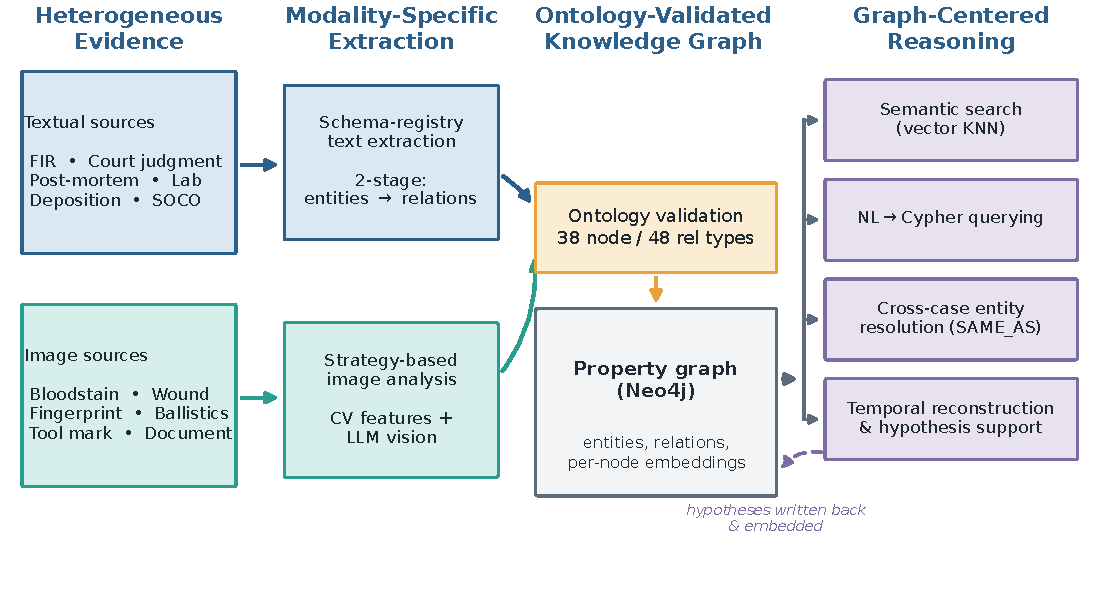
\includegraphics[width=0.96\textwidth]{architecture.pdf}
  \caption{End-to-end architecture. Textual and visual evidence are extracted by
  modality-specific components, type-checked against the forensic ontology,
  materialised in an embedded property graph, and consumed by semantic search,
  NL-to-Cypher querying, cross-case entity resolution, temporal reconstruction,
  and hypothesis support. Derived artefacts are written back and embedded.}
  \label{fig:arch}
\end{figure*}

\subsection{Ontology-Guided Forensic Knowledge Graph}
\label{sec:ontology}

The ontology is the backbone of the framework. It defines six semantic groups of
node types (core case, legal/judicial, medical/laboratory, scene/procedural,
forensic-image, and reasoning entities) together with the typed relationships
that connect them (\cref{fig:ontology}, \cref{tab:ontology}). Core case entities
(\node{Case}, \node{Person}, \node{Location}, \node{Evidence}, \node{Weapon},
\node{TimeEvent}, \dots) anchor every case. Legal entities (\node{LegalSection},
\node{Verdict}, \node{CourtOrder}) capture judicial structure; medical and
laboratory entities (\node{InjuryPattern}, \node{CauseOfDeath},
\node{ToxicologyResult}, \node{DNAProfile}, \dots) capture forensic-medical
findings; scene/procedural entities (\node{CrimeScene}, \node{PhysicalEvidence},
\node{ChainOfCustody}, \node{Statement}) capture investigative process; and
image entities (\node{BloodstainPattern}, \node{FingerprintPattern},
\node{WoundPattern}, \node{BallisticsPattern}, \node{ToolMarkPattern}, \dots)
capture visual analysis outputs. Reasoning entities (\node{Hypothesis},
\node{ImpactMechanismNode}, \node{Experiment}) host derived knowledge.

\begin{figure*}[t]
  \centering
  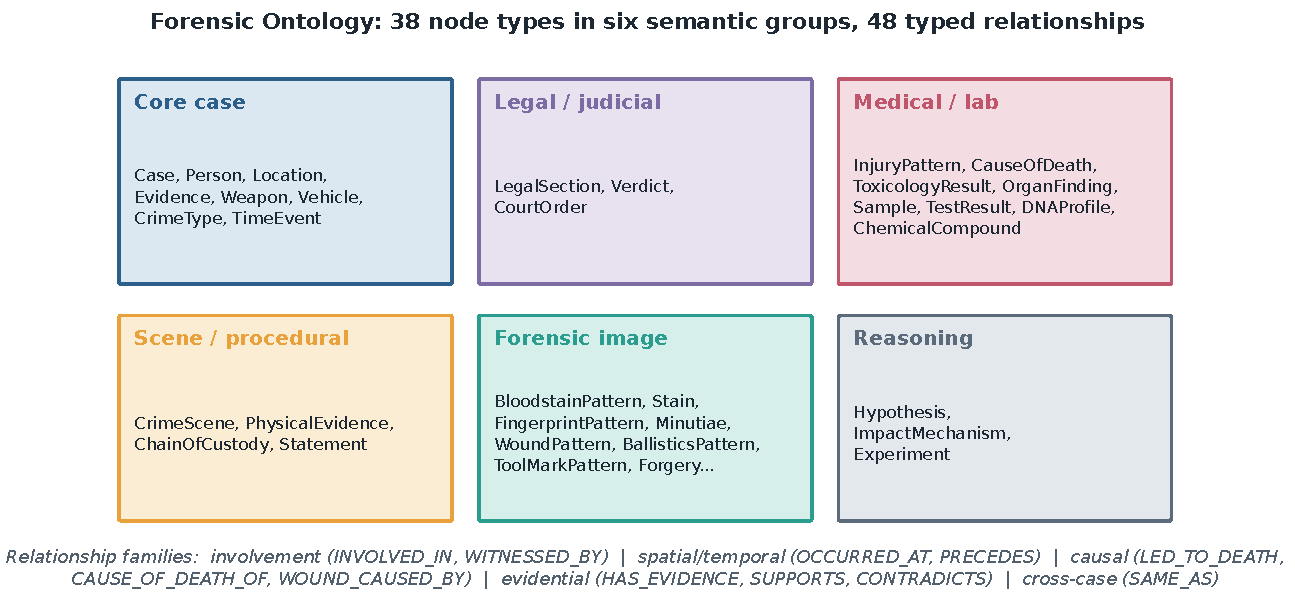
\includegraphics[width=0.94\textwidth]{ontology_overview.pdf}
  \caption{The forensic ontology groups 38 node types into six semantic
  families and connects them with 48 typed relationships organised into
  involvement, spatial/temporal, causal, evidential, image-derived, and
  cross-case families.}
  \label{fig:ontology}
\end{figure*}

% Ontology node-group summary (spans both columns)
\begin{table*}[t]
  \centering
  \caption{The forensic ontology organises 38 node types into six semantic
  groups and connects them with 48 typed relationships. Required properties and
  controlled enumerations (e.g.\ \texttt{PatternType}, \texttt{InjuryType},
  \texttt{FingerprintClass}) are enforced at insertion time.}
  \label{tab:ontology}
  \small
  \begin{tabular}{@{}P{2.6cm} c P{11.2cm}@{}}
    \toprule
    \textbf{Semantic group} & \textbf{\# types} & \textbf{Representative node types} \\
    \midrule
    Core case        & 8 & \texttt{Case}, \texttt{Person}, \texttt{Location}, \texttt{Evidence}, \texttt{Weapon}, \texttt{Vehicle}, \texttt{CrimeType}, \texttt{TimeEvent} \\
    Legal / judicial & 3 & \texttt{LegalSection}, \texttt{Verdict}, \texttt{CourtOrder} \\
    Medical / lab    & 8 & \texttt{InjuryPattern}, \texttt{CauseOfDeath}, \texttt{ToxicologyResult}, \texttt{OrganFinding}, \texttt{Sample}, \texttt{TestResult}, \texttt{DNAProfile}, \texttt{ChemicalCompound} \\
    Scene / procedural & 4 & \texttt{CrimeScene}, \texttt{PhysicalEvidence}, \texttt{ChainOfCustody}, \texttt{Statement} \\
    Forensic image   & 12 & \texttt{BloodstainPattern}, \texttt{Stain}, \texttt{FingerprintPattern}, \texttt{MinutiaePoint}, \texttt{RidgeDetail}, \texttt{WoundPattern}, \texttt{TissueAnalysis}, \texttt{BallisticsPattern}, \texttt{HandwritingFeature}, \texttt{InkAnalysis}, \texttt{ForgeryIndicator}, \texttt{ToolMarkPattern} \\
    Reasoning        & 3 & \texttt{Hypothesis}, \texttt{ImpactMechanismNode}, \texttt{Experiment} \\
    \midrule
    \multicolumn{3}{@{}P{15.5cm}@{}}{\textit{Relationship families:} involvement (\texttt{INVOLVED\_IN}, \texttt{WITNESSED\_BY}, \texttt{PRESIDED\_BY}); spatial/temporal (\texttt{OCCURRED\_AT}, \texttt{HAPPENED\_ON}, \texttt{PRECEDES}, \texttt{FOLLOWS}); causal/medical (\texttt{LED\_TO\_DEATH}, \texttt{CAUSE\_OF\_DEATH\_OF}, \texttt{WOUND\_CAUSED\_BY}, \texttt{INJURY\_CAUSED\_BY}); evidential (\texttt{HAS\_EVIDENCE}, \texttt{SUPPORTS}, \texttt{CONTRADICTS}, \texttt{CORROBORATES}); image-derived (\texttt{HAS\_PATTERN}, \texttt{HAS\_MINUTIAE}, \texttt{FIRED\_FROM}); and cross-case (\texttt{SAME\_AS}).} \\
    \bottomrule
  \end{tabular}
\end{table*}


Ontology validation is what separates this framework from unconstrained LLM
extraction. Graph construction is a left fold of a validated-insertion operator
$\oplus$ over the per-document and per-image subgraphs:
\begin{equation}
G \;=\; \Big(\bigoplus_i (V_{d_i},E_{d_i})\Big) \,\oplus\, \Big(\bigoplus_j (V_{x_j},E_{x_j})\Big),
\label{eq:construct}
\end{equation}
where $\oplus$ inserts only the valid nodes $\{v:\mathrm{valid}(v)\}$ and
admissible edges $\{e:\mathrm{adm}(e)\}$ of \cref{eq:valid,eq:adm}, coercing each
admitted node's properties to their declared types and merging nodes that share a
type's unique key. The invariant ``$G$ contains only valid nodes and admissible
edges'' therefore holds after every insertion. Two benefits follow. First,
\emph{reliability}: malformed or hallucinated structures are rejected before they
reach the store, so reasoning operates over a consistent representation. Second,
\emph{query safety}: because the schema is fixed, generated queries can be
grounded in real labels and edge patterns (\cref{sec:retrieval}) and a static
guard can reject destructive operations.

\subsection{Multi-Document Text Extraction}
\label{sec:text}

Text extraction maps six structurally different document types onto the same
graph target through a \emph{schema registry} (\cref{tab:registry}). Each source
type $s$ is associated with an entity schema, a relationship schema, and a
specialised system prompt.
Extraction proceeds in two stages
(\cref{alg:text}): first, entities are extracted under the entity schema with the
document-type prompt; second, relationships are extracted \emph{conditioned on
the already-identified entities}, so that the model links real referents rather
than inventing endpoints. Both stages use strict structured output constrained to
the schema, and every relationship is required to carry the text span that
supports it, enabling provenance and auditability.

The two-stage decomposition matters: relationship extraction is the harder,
more error-prone step, and grounding it in a fixed entity set both reduces the
combinatorial space and prevents the model from introducing entities through the
back door of a relationship. Document-type prompts inject domain knowledge
(e.g.\ that a post-mortem's deceased subject is a \node{Person} with a victim
role, that a \node{CauseOfDeath} should be linked to that person via
\rel{cause\_of\_death\_of}), while the common graph target guarantees that
heterogeneous documents become interoperable subgraphs.

\begin{algorithm}[t]
\caption{Two-stage, schema-constrained text extraction}
\label{alg:text}
\begin{algorithmic}[1]
\Require document $d$, source type $s$, ontology $O$, registry $\mathcal{R}$
\Ensure validated subgraph $(V_d,E_d)$
\State $(\Pi_{\text{ent}},\Sigma_{\text{ent}}) \gets \mathcal{R}[s]$
  \Comment{prompt + entity schema}
\State $\tilde V \gets \textsc{LLM}(\Pi_{\text{ent}},d)$ constrained to $\Sigma_{\text{ent}}$
\State $V_d \gets \{\,\textsc{Coerce}(v,O) : v\in\tilde V,\ \textsc{Valid}(v,O)\,\}$
\State $(\Pi_{\text{rel}},\Sigma_{\text{rel}}) \gets \mathcal{R}[s]$
\State $\tilde E \gets \textsc{LLM}(\Pi_{\text{rel}}, d, \textsc{Summary}(V_d))$ constrained to $\Sigma_{\text{rel}}$
\State $E_d \gets \{\, e\in\tilde E : \textsc{TypeCheck}(e,O)\ \wedge\ \mathrm{ends}(e)\subseteq V_d \,\}$
\State \textsc{PrefixIds}$(V_d,E_d,\mathit{docid})$ \Comment{namespace per document}
\State \Return $(V_d,E_d)$
\end{algorithmic}
\end{algorithm}

\begin{table}[t]
  \centering
  \caption{The schema registry binds each document type to an entity schema, a
  relation schema, and a prompt; all share the common graph target. Key entity
  types and a representative relation are shown.}
  \label{tab:registry}
  \footnotesize
  \setlength{\tabcolsep}{3.5pt}
  \begin{tabular}{@{}P{1.4cm}P{2.65cm}P{3.05cm}@{}}
    \toprule
    \textbf{Source type} & \textbf{Key entity types} & \textbf{Example relation} \\
    \midrule
    FIR & Case, Person, Location, Weapon, Evidence, TimeEvent & \rel{involved\_in} \\
    Court judgment & Person, LegalSection, Verdict, CourtOrder & \rel{charged\_under} \\
    Post-mortem & InjuryPattern, CauseOfDeath, ToxicologyResult & \rel{led\_to\_death} \\
    Lab report & Sample, TestResult, DNAProfile, Compound & \rel{matches\_dna} \\
    Deposition & Statement, Person, TimeEvent & \rel{stated\_by} \\
    SOCO & CrimeScene, PhysicalEvidence, ChainOfCustody & \rel{collected\_by} \\
    \bottomrule
  \end{tabular}
\end{table}

\subsection{Hybrid Forensic Image Analysis}
\label{sec:image}

Each image modality is handled by a strategy implementing a common four-stage
map $f_{\text{img}}=\textsc{build}\circ\textsc{combine}\circ\langle\textsc{cv},
\textsc{vision}\rangle$. The \textsc{cv} stage runs classical computer vision
(e.g.\ CLAHE enhancement, Otsu segmentation, and contour-based geometric and
spatial feature extraction for bloodstain images), producing the feature vector
$z_x$. The \textsc{vision} stage queries an LLM vision model with a domain prompt;
\textsc{combine} synthesises $z_x$, the vision output, and any experiment
metadata into a structured assessment; and \textsc{build} maps that assessment to
ontology-typed entities and relationships. The CV stage contributes quantitative
per-stain geometry and spatial statistics to the graph; an ablation
(\cref{sec:results}) finds that, on our impact-spatter sample, the LLM vision step
alone already detects the pattern, so the hybrid's CV features add graph structure
rather than classification accuracy on that coarse label.

\Cref{tab:imgmod} summarises the six modalities, the CV features each computes,
the semantic output produced, and the ground truth against which it is evaluated.
We stress an honest point that the evaluation (\cref{sec:results}) makes
quantitative: only some image types have ground truth that actually encodes the
attribute the task requires. Bloodstain analysis is evaluated against a
physics-grounded impact-spatter dataset; fingerprint labels in the public dataset
encode hand and finger \emph{position}, not pattern class, so they cannot
validate pattern recognition. We retain all six modalities in the framework but
report their evaluation faithfully.

\begin{table}[t]
  \centering
  \caption{Forensic image modalities: classical CV features, semantic output,
  and the ground truth used for evaluation. Alignment varies by modality and is
  quantified in \cref{tab:imgresults}.}
  \label{tab:imgmod}
  \scriptsize
  \setlength{\tabcolsep}{3.5pt}
  \begin{tabular}{@{}P{1.3cm}P{2.45cm}P{1.7cm}P{1.85cm}@{}}
    \toprule
    \textbf{Modality} & \textbf{CV features} & \textbf{Semantic output} & \textbf{Eval.\ target} \\
    \midrule
    Bloodstain & CLAHE, Otsu; geometry, spatial stats & pattern + mechanism & impact-spatter (aligned) \\
    Fingerprint & ridge, minutiae cues & pattern class & hand, finger (misaligned) \\
    Wound & region, colour cues & wound type + mechanism & present / absent (partial) \\
    Ballistics & striation cues & caliber, rifling & caliber (proxy) \\
    Document & layout, ink cues & forgery indicators & genuine / forged (hard) \\
    Tool marks & striation, impression cues & tool class & tool type (misaligned) \\
    \bottomrule
  \end{tabular}
\end{table}

\subsection{Multimodal Fusion}
\label{sec:fusion}

Fusion (\cref{fig:workflow}) inserts both branches' outputs into a single case
graph. Text and image subgraphs share the case namespace, and the fusion operator
adds cross-reference edges where a textual entity and an image-derived finding
co-refer (for example, a \node{Weapon} mentioned in an FIR and a
\node{BallisticsPattern} extracted from a fired-cartridge image, linked via
\rel{fired\_from}; or a \node{WoundPattern} from a wound image linked to the
weapon that a post-mortem attributes it to via \rel{wound\_caused\_by}). Because
the two branches are independent, fusion degrades gracefully: a text-only case
still yields a valid case graph, as does an image-only case. This robustness is a
direct consequence of the shared ontology: each branch produces typed,
self-contained structure that the graph can absorb in isolation or together.

\begin{figure*}[t]
  \centering
  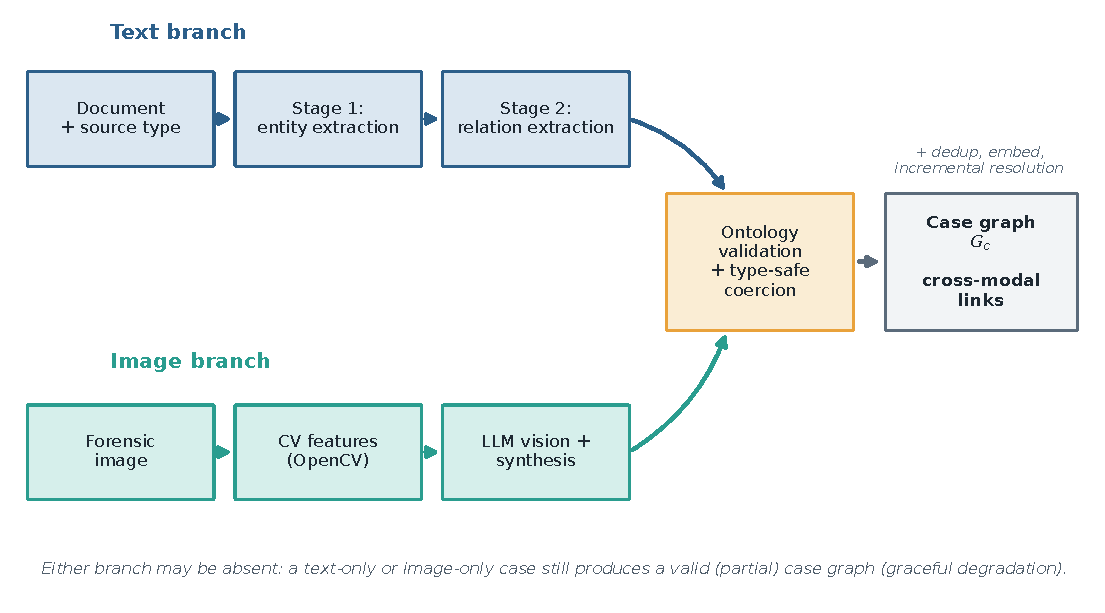
\includegraphics[width=0.92\textwidth]{multimodal_workflow.pdf}
  \caption{Multimodal extraction workflow. The text branch performs two-stage
  entity/relation extraction; the image branch fuses CV features with LLM vision.
  Both pass through ontology validation before insertion into the case graph
  $G_c$; either branch may be absent (graceful degradation).}
  \label{fig:workflow}
\end{figure*}

\subsection{Semantic Retrieval and NL-to-Graph Querying}
\label{sec:retrieval}

Each node is serialised by $\sigma$ and embedded by $\phi$, giving
$X(v)=\phi(\sigma(v))\in\mathbb{R}^{1536}$; a single cosine vector index over a
shared label covers all node types. Two capabilities follow. \emph{Semantic
search} returns, for a query $q$, the $k$ nearest nodes
\begin{equation}
\mathcal{N}_k(q)=\operatorname*{arg\,top\text{-}k}_{v\in V}\ \cos\!\big(\phi(q),X(v)\big),
\quad \cos(a,b)=\frac{\langle a,b\rangle}{\lVert a\rVert\,\lVert b\rVert}.
\label{eq:knn}
\end{equation}
\emph{Grounded NL-to-graph querying} conditions generation on real graph content.
From $\mathcal{N}_k(q)$ we collect the retrieved nodes' stored property values and
the set of \emph{realised} schema edges
\begin{equation}
\begin{split}
\mathcal{P}(\mathcal{N}_k)=\big\{(\tau(u),r,\tau(w)) :\ &(u,r,w)\in E,\\[-1pt]
&\{u,w\}\cap\mathcal{N}_k\neq\varnothing\big\},
\end{split}
\label{eq:patterns}
\end{equation}
and pass $(q,\text{props},\mathcal{P})$ to the generator, so it filters on values
that exist and traverses edges that exist, e.g.\
\texttt{(:InjuryPattern)-[:LED\_TO\_DEATH]->(:CauseOfDeath)}, rather than
hypothesising schema. A bounded loop repairs an erroneous query by returning the
database error to the generator (at most a few attempts), and a static guard
rejects destructive operations. These are means to grounded, trustworthy
querying rather than contributions in themselves.

\subsection{Cross-Case Entity Resolution}
\label{sec:resolution}

Each document is extracted into its own namespace, so the same real-world
entity (a recurring judge, a shared location, a weapon type) appears as
distinct nodes across cases. Resolution links these without merging them
(\cref{fig:resolution}, \cref{alg:resolve}).

\textbf{Blocking.} Rather than comparing all $\Theta(n^2)$ cross-namespace pairs,
we restrict comparison to the candidate set
\begin{equation}
\mathcal{B}=\big\{(i,j): \mathrm{ns}(i)\neq\mathrm{ns}(j),\ \cos(X_i,X_j)\ge\theta_{\text{block}}\big\},
\label{eq:block}
\end{equation}
using the node embeddings of \cref{eq:knn} to keep only semantically near pairs.

\textbf{Verification.} Let $\nu$ normalise a name (lowercasing; stripping
honorifics, role words, and non-alphanumerics). For $(i,j)\in\mathcal{B}$ let
$\sigma_{ij}\in[0,1]$ be the normalised-name similarity (a sequence-overlap ratio
with a subset bonus for multi-token containment), $\rho_{ij}=\mathbf{1}[r_i=r_j]$
role agreement, and
\begin{equation}
\omega_{ij}=\frac{|\mathrm{ctx}_i\cap\mathrm{ctx}_j|}{|\mathrm{ctx}_i\cup\mathrm{ctx}_j|}
\label{eq:jaccard}
\end{equation}
the Jaccard overlap of the nodes' 2-hop context bags (neighbour names, excluding
\node{Case} and \rel{same\_as}). The pair is accepted iff
\begin{equation}
\sigma_{ij}\ge\theta_{\text{name}}\ \wedge\ \big(\mathrm{unamb}(i,j)\vee\omega_{ij}>0\vee\mathrm{distinct}(r_i,r_j)\big),
\label{eq:accept}
\end{equation}
where $\mathrm{unamb}$ holds when the shorter name is multi-token with no
conflicting initials and $\mathrm{distinct}$ holds when both share a recurring
distinctive role (judge, investigating officer). Weak signals (single-token or
common names, conflicting initials) therefore cannot link without corroborating
context or role.

\textbf{Non-destructive linking.} An accepted pair receives a transparent
confidence
\begin{equation}
c_{ij}=0.6\,\sigma_{ij}+0.25\min(\omega_{ij},1)+0.15\,\rho_{ij}
\label{eq:conf}
\end{equation}
and is joined by an edge $i\xrightarrow{\rel{same\_as}\{c_{ij}\}}j$; connected
components (union--find) yield cross-case clusters. Because $|V|$ is unchanged,
provenance is preserved exactly: no node is merged or deleted. This reflects a
forensic priority, a false merge fabricates a connection between unrelated cases
and is far more damaging than a missed link.

\begin{figure*}[t]
  \centering
  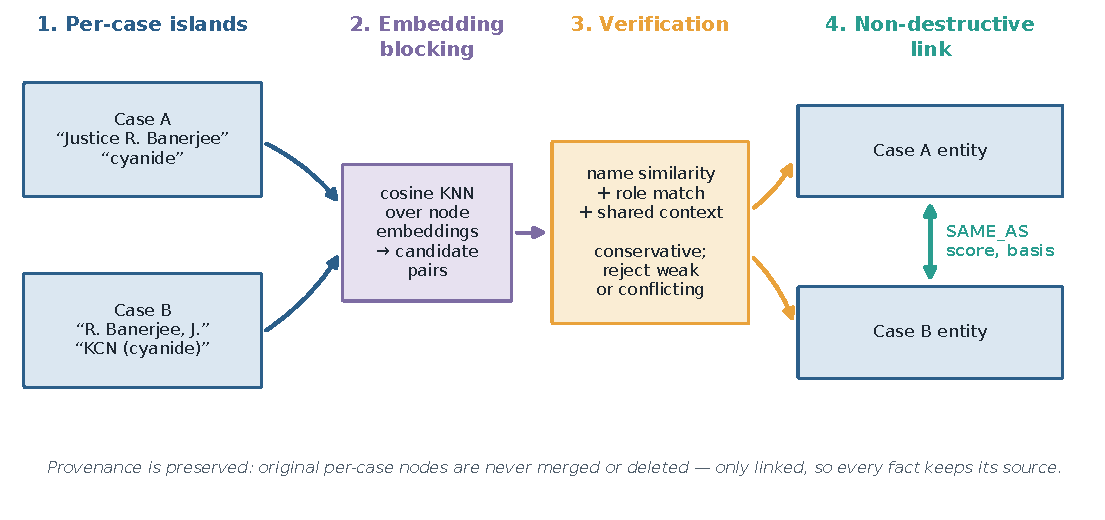
\includegraphics[width=0.94\textwidth]{entity_resolution.pdf}
  \caption{Cross-case entity resolution. Per-case islands are compared via
  embedding-blocked candidate generation, verified by name/role/context, and
  linked with non-destructive \rel{same\_as} edges that preserve provenance.}
  \label{fig:resolution}
\end{figure*}

\begin{algorithm}[t]
\caption{Incremental, non-destructive cross-case resolution}
\label{alg:resolve}
\begin{algorithmic}[1]
\Require new namespace $p$; resolvable labels $L$; thresholds $\theta_{\text{block}},\theta_{\text{name}}$
\Ensure \rel{same\_as} links connecting namespace $p$ to the rest of $G$
\State $\Lambda \gets \varnothing$
\For{each label $\ell \in L$}
  \State $N \gets$ $\ell$-nodes with embedding $X$, role $r$, 2-hop context $\mathrm{ctx}$
  \State normalise names via $\nu$; discard generic placeholders
  \For{each new node $i\in N$ with $\mathrm{ns}(i)=p$} \Comment{$\Theta(|p|\cdot|N|)$}
    \For{each node $j\in N$ with $\mathrm{ns}(j)\neq p$}
      \If{$\cos(X_i,X_j) < \theta_{\text{block}}$} \textbf{continue} \Comment{blocking, \cref{eq:block}}
      \EndIf
      \State compute $\sigma_{ij}$, $\omega_{ij}$ (\cref{eq:jaccard}), $\rho_{ij}$
      \If{$(i,j)$ accepted by \cref{eq:accept}}
        \State $c_{ij}\gets$ confidence (\cref{eq:conf})
        \State $\Lambda \gets \Lambda \cup \{\, i\xrightarrow{\rel{same\_as}\{c_{ij}\}} j \,\}$
      \EndIf
    \EndFor
  \EndFor
\EndFor
\State \Return $\Lambda$
\end{algorithmic}
\end{algorithm}

\subsection{Temporal Reasoning and Hypothesis Support}
\label{sec:temporal}

The prototype includes a temporal reasoning module over \node{TimeEvent} nodes
attached to a case. As \cref{sec:results} reports, the pipeline recovers the
documented dates well (\node{TimeEvent} $\mathrm{F1}=0.88$, date coverage $0.95$),
so this module operates on reliable dated events. The analyser parses heterogeneous
timestamp strings, orders events chronologically, computes the overall time span,
and flags inconsistencies, large gaps between consecutive events and
contradictions between explicit \rel{precedes}/\rel{follows} edges and parsed
timestamps. Such gaps and contradictions are exactly the cues an
investigator looks for (an unexplained interval, a statement that is
chronologically impossible).

Hypothesis support retrieves a case's connected evidence (persons, locations,
patterns, mechanisms, and (for bloodstain experiments) per-stain statistical
features) and asks an LLM to produce a primary hypothesis with explicit
supporting and contradicting evidence, alternative hypotheses, and a reasoning
chain. The hypothesis is stored as a \node{Hypothesis} node linked to the case
and embedded, so it becomes part of the queryable, semantically searchable graph.
We emphasise the framing: the system produces \emph{auditable hypothesis support},
not a verdict. Every hypothesis points back to the specific evidence nodes
behind it (\cref{fig:chain}), so a human analyst can inspect, accept, or reject
it on the basis of the cited evidence.

\begin{figure*}[t]
  \centering
  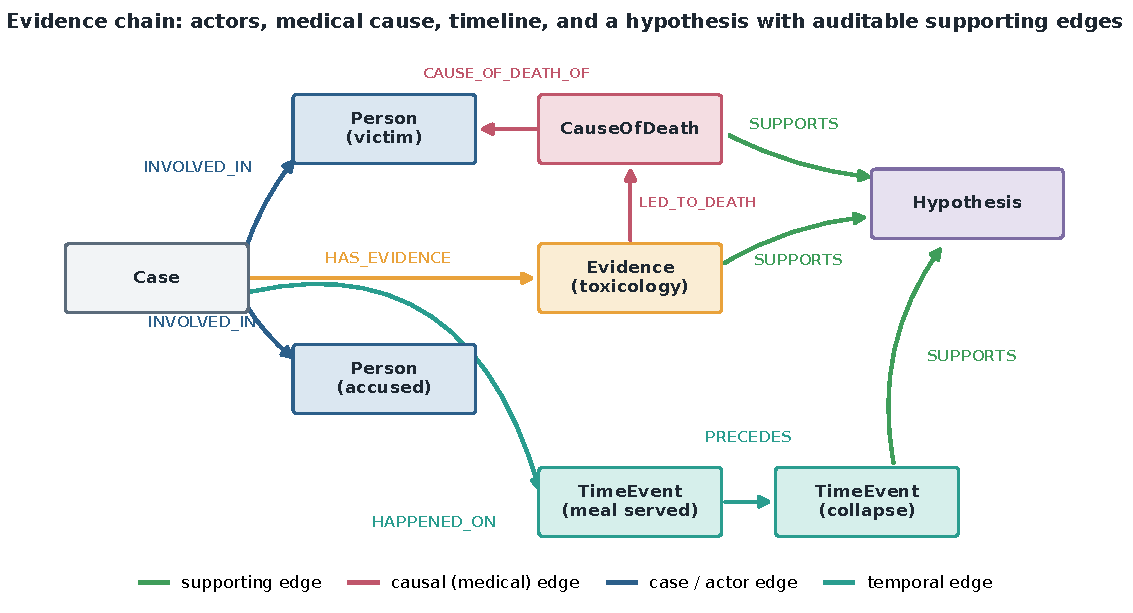
\includegraphics[width=0.9\textwidth]{evidence_chain.pdf}
  \caption{An example evidence chain. A hypothesis is connected to the specific
  toxicology evidence, medical cause of death, and timeline events that support
  it; supporting and contradicting edges make the reasoning auditable.}
  \label{fig:chain}
\end{figure*}

% =====================================================================
\section{Implementation}
\label{sec:impl}

The framework is realised as a prototype used solely to obtain the measurements
reported here; none of the contribution depends on these choices. Extraction and
reasoning run in Python; the typed graph and its cosine vector index are stored
in Neo4j~\cite{neo4j}; classical image features use OpenCV~\cite{bradski2000opencv};
and extraction, embedding, and vision calls use a hosted LLM. Interface details
are immaterial to the research questions and are omitted.

% =====================================================================
\section{Experimental Setup}
\label{sec:setup}

% Dataset summary (spans both columns)
\begin{table*}[t]
  \centering
  \caption{Datasets used for development and evaluation. Synthetic gold is useful
  for regression testing but circular for validity; documented real cases and
  physics-grounded image data provide the stronger external evidence.}
  \label{tab:datasets}
  \small
  \begin{tabular}{@{}P{3.2cm} P{2.7cm} r P{4.3cm} P{3.6cm}@{}}
    \toprule
    \textbf{Dataset} & \textbf{Source} & \textbf{Items} & \textbf{Role / modality} & \textbf{Ground-truth alignment} \\
    \midrule
    Indian court judgments & Public records / HF~\cite{indiancourt} & 38 & Real legal text extraction & Document text (no per-entity gold) \\
    Documented real cases  & Court records / public sources & 28 & Real-case entity validation & Two-annotator documented facts \\
    Synthetic FIR / PM / lab / deposition / SOCO & LLM-generated & 120 & Text extraction regression & Self-consistent (circular) \\
    Attinger bloodstain~\cite{attinger2018bloodstain} & Published (2018) & 61 exp. & Bloodstain image analysis & Physics-grounded mechanism \\
    SOCOFing~\cite{socofing} & Kaggle & 110{,}540 & Fingerprint image analysis & Hand/finger label (not pattern class) \\
    CEDAR signatures~\cite{cedar2004signature} & Public release & 2{,}640 & Document forgery detection & Genuine vs.\ forged \\
    AZH wounds~\cite{azhwound} & Public release & 1{,}867 & Wound image analysis & Clinical class (not forensic type) \\
    Synthetic ballistics / tool marks & Procedurally generated & 40 & Image analysis regression & Known synthetic parameters \\
    \bottomrule
  \end{tabular}
\end{table*}


\subsection{Datasets}
\Cref{tab:datasets} summarises the data. For text we use real Indian court
judgments~\cite{indiancourt}; 28 well-documented real Indian criminal cases with
human-curated factual gold (e.g.\ the Koodathayi cyanide killings and the 2024
R.G.\ Kar case), curated from authoritative public sources; and synthetic FIR,
post-mortem, laboratory, deposition, and SOCO reports used for regression. For
images we use the Attinger impact-spatter bloodstain
dataset~\cite{attinger2018bloodstain}, SOCOFing fingerprints~\cite{socofing},
CEDAR signatures~\cite{cedar2004signature}, AZH wound images~\cite{azhwound}, and
procedurally generated ballistics and tool-mark images.

\subsection{Two evaluation tracks}
\label{sec:tracks}
We separate two tracks with deliberately different epistemic status.
\emph{Track~1: synthetic-gold regression.} The 120 synthetic FIR, post-mortem,
laboratory, deposition, and SOCO documents carry LLM-generated gold. Because the
gold and the system under test are the same class of model, agreement measures
\emph{self-consistency}, not correctness; we use it only to detect regressions and
never report it as external evidence.
\emph{Track~2: real-case validation (primary).} The 28 well-documented cases
carry gold curated from authoritative public records, documented facts not
produced by any LLM. A first annotator curated the gold from the cited sources
(dropping two unnatural-death cases as edge cases of non-canonical crime type, and
normalising entries such as name spellings and the principal location); a
\emph{second} annotator then independently re-annotated all 28 cases blind to the
first. Inter-annotator agreement is high: Cohen's $\kappa=0.95$ on person roles
and $1.0$ on crime type (\cref{sec:iaa}, \cref{tab:iaa}), which validates the
first annotator's curation as the gold used here; the full disagreement list is
released for adjudication. The pipeline extracts entities from a factual narrative and
is scored against those facts. This is our \textbf{primary} result because it
breaks the circularity of Track~1.

\subsection{Matching and image metrics}
Real-case matching is type-specific: persons, locations, and weapons use fuzzy
string matching; crime type uses canonical-keyword matching against the case
description (where the FIR extractor records the crime); and timeline events use
date-aware matching on extracted year/month against documented dates, so
descriptively named events are compared fairly to dated gold. Image analysis uses
per-attribute accuracy for categorical attributes, precision/recall/F1 for binary
attributes, and mean absolute error for numeric attributes, and is \emph{stratified
by ground-truth alignment}: aligned (bloodstain, physics-grounded), proxy
(ballistics caliber), and misaligned (fingerprint hand/finger labels for a
pattern-class task). A methodological safeguard is a \emph{label-free} item
identifier: the filename stem in several public datasets encodes the ground-truth
label, so passing it as metadata would leak the answer into the prompt; removing
this leak corrected an early, falsely perfect fingerprint result
(\cref{sec:results}).

\subsection{Configuration and reproducibility}
\label{sec:config}
Unless stated otherwise, extraction uses GPT-4.1 with strict JSON-schema
structured outputs (falling back to JSON-object mode where the schema mode is
unsupported) at decoding temperature $0.1$; node embeddings are
$1536$-dimensional. We report the mean (and standard deviation) over \emph{three}
independent runs per condition, plus a case-level bootstrap $95\%$ CI over the $28$
cases (\cref{sec:results}); at this temperature all types are stable
(F1 sd $\le 0.03$, and $\le0.01$ for all but \node{Location}). Cross-case resolution uses an embedding blocking floor
$\theta_{\text{block}}=0.78$ and a name threshold $\theta_{\text{name}}=0.88$
(\cref{eq:block,eq:accept}). The exact 28-case list, their public sources, gold
composition, per-case scores, and the curator-plus-review curation protocol are given in
\cref{app:cases}; the documented-fact gold and the experiment scripts are released
with the paper.

\subsection{Controlled comparisons}
\label{sec:baselines}
We run three controlled ablations: ontology-guided extraction vs.\ a naive,
same-LLM JSON baseline (\cref{sec:ablation}), which isolates the schema guidance
of \cref{eq:valid,eq:adm}; a CV-only vs.\ LLM-only vs.\ CV$+$LLM ablation of
the bloodstain image pipeline (\cref{sec:results}); and a grounded vs.\ ungrounded
NL-to-Cypher ablation of the reasoning layer (\cref{tab:queryabl}). The remaining
single-component comparisons (removing the graph entirely and
disabling resolution, \cref{eq:accept}) are left to future work
(\cref{sec:future}); we report measured ablations, not the full matrix, rather
than approximate the rest with unmeasured numbers.

% =====================================================================
\section{Results}
\label{sec:results}

\Cref{tab:rqs} maps each research question to its evidence and headline finding;
the subsections that follow elaborate each in turn.

\begin{table}[t]
  \centering
  \caption{Research questions, supporting evidence, and main findings.}
  \label{tab:rqs}
  \footnotesize
  \setlength{\tabcolsep}{3.5pt}
  \begin{tabular}{@{}P{0.6cm}P{2.0cm}P{4.5cm}@{}}
    \toprule
    \textbf{RQ} & \textbf{Evidence} & \textbf{Main finding} \\
    \midrule
    RQ1 & ablation (\cref{fig:ablation}) & ontology guidance lifts macro-F1 $0.53\!\to\!0.73$ and recovers \node{Weapon} $0.00\!\to\!0.72$ \\
    RQ2 & \cref{sec:tracks}, \cref{tab:realcase} & synthetic gold is consistency-only; real-case micro-F1 $0.78$ (CI $[0.74,0.82]$, $n{=}28$) \\
    RQ3 & \cref{tab:imgresults} & only bloodstain has task-aligned ground truth (F1 $1.0$, full set $n{=}61$) \\
    RQ4 & \cref{sec:res_eval}, \cref{tab:resolution,tab:frontier} & precision-oriented \rel{same\_as}: \emph{instance-identity} P$0.92$/R$0.79$ (shared suspects, agencies), separable from category normalization; $1$ common-name merge \\
    \bottomrule
  \end{tabular}
\end{table}

\subsection{Synthetic regression (consistency check, not headline)}
On the 120 synthetic documents the pipeline reproduces the LLM-generated gold
with consistently high, stable agreement across runs, and every extracted
structure satisfies the ontology (\cref{eq:valid,eq:adm}). Per \cref{sec:tracks},
this is a regression signal only: it confirms stability and schema compliance but
says nothing about real-world correctness, so we do not interpret it as evidence
and report the real-case track below as our headline result.

\subsection{Real-case validation (primary result)}
\Cref{tab:realcase} and \cref{fig:f1} report the full system on the 28
documented cases (two-annotator gold, \cref{sec:iaa}; \cref{sec:setup}), averaged
over three independent runs. Person,
crime-type, weapon/method, and dated-event extraction are strong and \emph{stable}:
$\mathrm{F1}=0.88\pm0.01$, $0.91\pm0.01$, $0.72\pm0.01$, and $0.88\pm0.01$
respectively, with standard deviations at or below $0.01$. \node{TimeEvent}
matching scores against the structured \texttt{date} field, where the pipeline
records each event's calendar date in ISO form. The matching rule is deliberately
explicit: a gold date counts as recovered when the extracted date shares its
\emph{year}, refined to year-\emph{and}-month when both sides name a month;
day-level exactness is \emph{not} required. This year-or-year-month rule (rather
than exact-ISO matching) matches the gold's own granularity, several documented
dates are recorded year-only (e.g.\ a conviction in ``2003''), and the
\emph{identical} rule scores both the full system and the baseline, so it cannot
favour one. An earlier evaluation that read
only the free-text event \emph{name} (not the \texttt{date} field) under-counted
recovery at $\mathrm{F1}=0.09$, conflating ``stored in a separate field'' with
``not extracted'', exactly the schema-compliance-versus-validity distinction this
paper argues for (\cref{sec:erroranalysis}). \node{Location} is the one genuinely weak type
($\mathrm{F1}=0.27$) because the gold names a single principal location while the
narrative mentions many places. Overall micro-$\mathrm{F1}$ is $0.78$ ($\pm0.01$)
and macro-$\mathrm{F1}$ $0.73$ ($\pm0.01$); the small gap between them reflects that
only \node{Location} lags. We regard the strong, low-variance recovery of persons,
crime types, weapons, and dates on \emph{real} data, validated against documented
facts no synthetic benchmark could provide, as the substantive result. Per case,
full-system $\mathrm{F1}$ ranges from $0.60$ (Soumya, train) to $0.94$ (Dabholkar),
mean $0.78$ (\cref{tab:cases}). A case-level bootstrap ($B{=}2000$, resampling the
28 cases) places the $95\%$ confidence interval for overall $\mathrm{F1}$ at
$[0.74,0.82]$ (micro) and $[0.68,0.78]$ (macro).

To check whether the strict per-mention metrics understate practical usefulness,
we add two complementary measures. \emph{Principal-location recall} (does any
extracted location match the single gold principal location under the strict
fuzzy matcher?) is $0.39$ ($11/28$ cases); much of the gap to the precision-driven
$\mathrm{F1}$ ($0.27$) is additional, genuinely-mentioned locations counted as
false positives, and many ``misses'' are \emph{more specific} than the gold
(\cref{sec:erroranalysis}). The human inter-annotator study (\cref{sec:iaa}) shows
this is granularity, not error: two annotators name the same place but at different
specificity. Quantifying that, a \emph{granularity-tolerant} principal-location
recall, which credits the gold place when an extracted location names it at any
granularity (token superset or subset), reaches $\mathbf{0.86}$ ($24/28$). The
cases it credits over the strict matcher are the same place named more or less
specifically (``Vasant Vihar'' vs.\ ``Vasant Vihar, New Delhi''; ``Koodathayi''
vs.\ ``Koodathayi, Kozhikode''); it deliberately does \emph{not} credit genuine
mismatches (Chhaparvad vs.\ Randhikpur), and even under-counts, missing cases
where the system named only a sub-scene (``St Pius X Convent'' for Kottayam). The
system therefore recovers the correct principal place far more often
($\approx\!0.86$) than the strict per-mention metric ($0.27$) suggests; what it
lacks is \emph{principal-location selection}, not place recognition. A simple,
gold-free selector confirms this is fixable: taking the \emph{first-mentioned}
extracted location as the principal scene identifies it correctly in $21/28$ cases
($0.75$): a concrete, near-term improvement over the $0.27$ per-mention
$\mathrm{F1}$, though principal-location \emph{selection} (vs.\ place recognition)
remains the open problem (\cref{tab:locmetrics}).
\emph{Date coverage}, the fraction of documented years recovered anywhere in the
extracted timeline, is $0.95$, confirming that the pipeline does recover the
documented dates: the looser coverage metric and the corrected per-mention
\node{TimeEvent} score agree. The one genuinely weak type is \node{Location}:
partly a matching-design issue and partly a principal-location selection problem
(the system does not yet single out the principal scene from secondary places).

\begin{table}[t]
  \centering
  \caption{\node{Location} by metric. The strict per-mention F1 understates place
  recovery: the system finds the principal place at \emph{some} granularity $0.86$
  of the time, and a gold-free first-mention selector picks it correctly $0.75$ of
  the time. Principal-location \emph{selection}, not place recognition, is the
  open problem.}
  \label{tab:locmetrics}
  \footnotesize
  \setlength{\tabcolsep}{5pt}
  \begin{tabular}{@{}P{5.8cm}c@{}}
    \toprule
    \textbf{Location metric} & \textbf{Result} \\
    \midrule
    Per-mention F1 (strict)                          & 0.27 \\
    Principal-location recall (strict fuzzy)         & 0.39 \\
    Principal-location recall (granularity-tolerant) & 0.86 \\
    Principal-location selection (first-mention rule) & \textbf{0.75} \\
    \bottomrule
  \end{tabular}
\end{table}

\begin{table}[t]
  \centering
  \caption{Real-case validation (full system) on 28 documented Indian criminal
  cases (two-annotator gold): mean over three independent runs (gpt-4.1,
  temperature $0.1$); the F1 column reports mean\,$\pm$\,standard deviation. Scores
  are against human-curated documented facts, not LLM-generated gold.}
  \label{tab:realcase}
  \small
  \begin{tabular}{@{}lccc@{}}
    \toprule
    \textbf{Entity type} & \textbf{P} & \textbf{R} & \textbf{F1 (mean$\pm$sd)} \\
    \midrule
    Person          & 0.82 & 0.95 & \textbf{0.88}\,$\pm$\,0.01 \\
    CrimeType       & 0.89 & 0.94 & \textbf{0.91}\,$\pm$\,0.01 \\
    Weapon / method & 0.79 & 0.66 & 0.72\,$\pm$\,0.01 \\
    Location        & 0.19 & 0.44 & 0.27\,$\pm$\,0.03 \\
    TimeEvent       & 0.85 & 0.91 & \textbf{0.88}\,$\pm$\,0.01 \\
    \midrule
    \textbf{Overall (micro)} & 0.72 & 0.86 & \textbf{0.78}\,$\pm$\,0.01 \\
    \textbf{Overall (macro)} & 0.71 & 0.78 & 0.73\,$\pm$\,0.01 \\
    \bottomrule
  \end{tabular}
\end{table}

\begin{figure}[t]
  \centering
  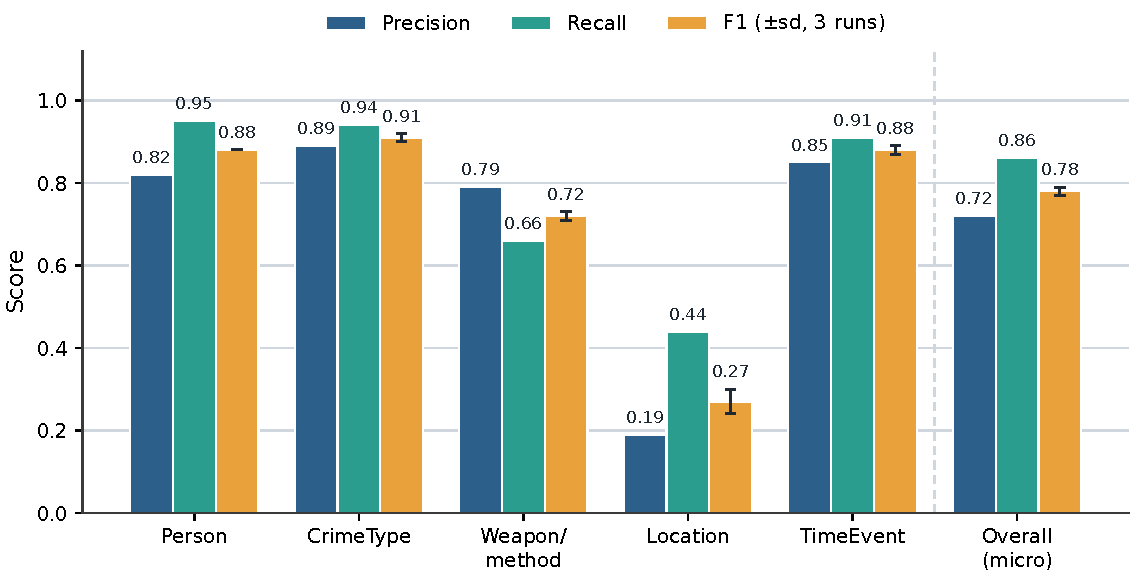
\includegraphics[width=\columnwidth]{real_case_f1.pdf}
  \caption{Full-system precision, recall, and F1 by entity type on the 28
  documented cases (mean over three runs; F1 error bars are $\pm$1 sd). Persons,
  crime types, weapons, and dated events are recovered strongly and stably;
  \node{Location} is the one weak type.}
  \label{fig:f1}
\end{figure}

\subsection{Inter-annotator agreement}
\label{sec:iaa}
To validate the documented-fact gold beyond a single curator, a second annotator
independently re-annotated all 28 cases from the case narratives, blind to the
first annotator's gold; \cref{tab:iaa} reports agreement. On the two genuinely
\emph{categorical} decisions, each shared person's role and each case's primary
crime type, Cohen's $\kappa$ is $0.95$ and $1.0$ (``almost perfect'' and
``perfect'' on the Landis--Koch scale). On the open-set mention categories, where
$\kappa$ is degenerate (no closed true-negative universe) and pairwise
$\mathrm{F1}$ is the standard agreement metric, agreement is high for
\node{Person} ($0.86$), \node{CrimeType} ($0.97$), \node{TimeEvent} ($0.93$), and
\node{Weapon} ($0.75$). \node{Location} agreement is \emph{low} ($0.36$), and
tellingly so: manual inspection shows the two annotators name the same place in
$16$ of $18$ ``disagreements,'' differing only in granularity (``Munirka'' vs.\
``a private bus in Munirka''; ``Bagiya restaurant'' vs.\ ``Bagiya barbecue
restaurant, Ashok Yatri Niwas hotel''). That two humans agree on the place yet
score $\mathrm{F1}=0.36$ is direct, human-grounded evidence that the system's low
\node{Location} score (\cref{sec:results}) is a metric/representation artefact, not
an extraction failure. The few genuine disagreements are defensible edge cases (a
witness who was also assaulted; a pathologist labelled \emph{officer} vs.\
\emph{forensic\_analyst}; a driver-turned-approver labelled \emph{witness} vs.\
\emph{accused}); they are documented in the released agreement report rather than
silently merged. The evaluation gold is the first annotator's curation, which this
high agreement validates; because the system metric matches person \emph{names}
(not roles), the few role disagreements do not affect the reported scores. One
caveat: the second annotator worked from the case narratives while the first
curated from the cited sources, so the agreement also spans that
source-to-narrative representation gap, which makes the reported $\kappa$ a
\emph{conservative} estimate of curation reliability rather than an inflated one.
A forensic-expert third pass (\cref{sec:future}) remains the natural next step.

\begin{table}[t]
  \centering
  \caption{Inter-annotator agreement on the 28-case gold (two independent
  annotators). Cohen's $\kappa$ for the categorical decisions; pairwise F1
  (positive specific agreement) for the open-set mention categories, where
  $\kappa$ does not apply.}
  \label{tab:iaa}
  \footnotesize
  \setlength{\tabcolsep}{5pt}
  \begin{tabular}{@{}lcc@{}}
    \toprule
    \textbf{Decision} & \textbf{Metric} & \textbf{Agreement} \\
    \midrule
    Person role        & Cohen's $\kappa$ & \textbf{0.95} \\
    Primary crime type & Cohen's $\kappa$ & \textbf{1.00} \\
    \midrule
    Person mention     & pairwise F1 & 0.86 \\
    CrimeType set      & pairwise F1 & 0.97 \\
    TimeEvent dates    & pairwise F1 & 0.93 \\
    Weapon             & pairwise F1 & 0.75 \\
    Location           & pairwise F1 & 0.36$^\dagger$ \\
    \bottomrule
    \multicolumn{3}{@{}l}{\footnotesize $^\dagger$Same place, different granularity in $16/18$ cases (text).} \\
  \end{tabular}
\end{table}

\subsection{Faculty-supervised domain-plausibility review}
\label{sec:facultyreview}
Beyond the two-annotator gold, a faculty domain reviewer, \emph{not} a forensic or
legal practitioner, assessed the manuscript for research design, ontology
plausibility, and forensic/evidence-structuring relevance. The review judged the
node categories (\node{Case}, \node{Person}, \node{Location}, \node{Evidence},
\node{Weapon}, \node{TimeEvent}, \node{InjuryPattern}, \node{CauseOfDeath},
\node{ToxicologyResult}, \node{DNAProfile}, \node{CrimeScene},
\node{ChainOfCustody}, \node{Statement}, and the image-derived patterns)
\emph{broadly plausible} for evidence-centric case modelling, and the relationship
families (involvement, spatial/temporal, causal/medical, evidential, image-derived,
and cross-case) \emph{appropriate} for forensic reasoning support. It found the
two-track evaluation and the two-annotator gold ($\kappa$ for categorical labels,
pairwise F1 for open sets) an appropriate methodological choice, the
granularity reading of the lower \node{Location} agreement reasonable, and the
conservative claim framing (decision/hypothesis support, not legally admissible
evidence or a replacement for experts) correct. We \emph{adopt} the review's
recommendations: keep claims at the level of a \emph{research prototype} and
validity-aware evaluation framework, and treat review by forensic/legal
\emph{practitioners}, a larger and less self-selected case set, stronger
principal-location adjudication, and an explicit mapping between Indian legal and
forensic-medical categories and the graph schema as future work
(\cref{sec:future}). We stress that this is a \emph{plausibility} review of the
design and ontology, not forensic-expert ground-truth validation of the labels,
which remains future work.

\subsection{Image analysis}
\Cref{tab:imgresults} and \cref{fig:imgeval} report image evaluation, and they
deliberately include negative results. Bloodstain impact-spatter recognition
reaches $\mathrm{F1}=1.0$ on the \emph{full} Attinger impact-spatter set
($n{=}61$, every sample scored, none skipped): the one modality with real,
physics-grounded ground truth. We still read this conservatively: it is a coarse
binary detection metric (the dataset is all impact-spatter, so there are no hard
negatives) on a single dataset and the prompt was not separately held out. It is
therefore evidence of full-set impact-spatter \emph{detection} on one dataset,
\emph{not} general bloodstain-pattern recognition or a broad image-forensics claim. Wound \emph{detection} (present vs.\ absent) over-detects
(recall $1.0$, precision $0.5$). Ballistics caliber is recovered at roughly
chance-level accuracy on synthetic data. The remaining tasks fail: single-image
document forgery detection is near zero because deciding genuineness generally
requires a reference exemplar; tool-mark tool-type classification is near zero on
synthetic marks; and fingerprint pattern recognition is near zero \emph{because
the dataset labels encode hand and finger position, not pattern class}, the
ground truth does not contain the attribute the task needs. We report these
faithfully: they are not defects to be hidden but a map of the framework's
operating envelope, and they expose a concrete evaluation-validity bug. The
label-leak fix of \cref{sec:setup} moved the \emph{reported} fingerprint score
from a false $100\%$ (the filename label leaking into the prompt) to an honest
$\approx\!0\%$: a swing that is itself evidence for why honest, leakage-free
evaluation matters.

\begin{table}[t]
  \centering
  \caption{Image evaluation, including honest negative results. ``Aligned''
  ground truth encodes the attribute the task requires; ``misaligned'' does not.
  $^\dagger$Full Attinger set ($n{=}61$); single-dataset, coarse binary
  detection metric.}
  \label{tab:imgresults}
  \footnotesize
  \setlength{\tabcolsep}{4pt}
  \begin{tabular}{@{}P{2.15cm}ccP{2.3cm}@{}}
    \toprule
    \textbf{Image task} & \textbf{Metric} & \textbf{Score} & \textbf{Ground-truth status} \\
    \midrule
    Bloodstain (impact spatter) & F1 & \textbf{1.00}$^\dagger$ & physics-grounded, aligned \\
    Wound (present/absent) & P/R & 0.50 / 1.00 & partial (over-detects) \\
    Ballistics (caliber) & acc. & $\approx$0.50 & proxy / synthetic \\
    Document (forgery) & F1 & $\approx$0 & hard (needs exemplar) \\
    Tool marks (tool type) & acc. & $\approx$0 & misaligned / synthetic \\
    Fingerprint (pattern) & acc. & $\approx$0 & misaligned labels \\
    \bottomrule
  \end{tabular}
\end{table}

\begin{figure}[t]
  \centering
  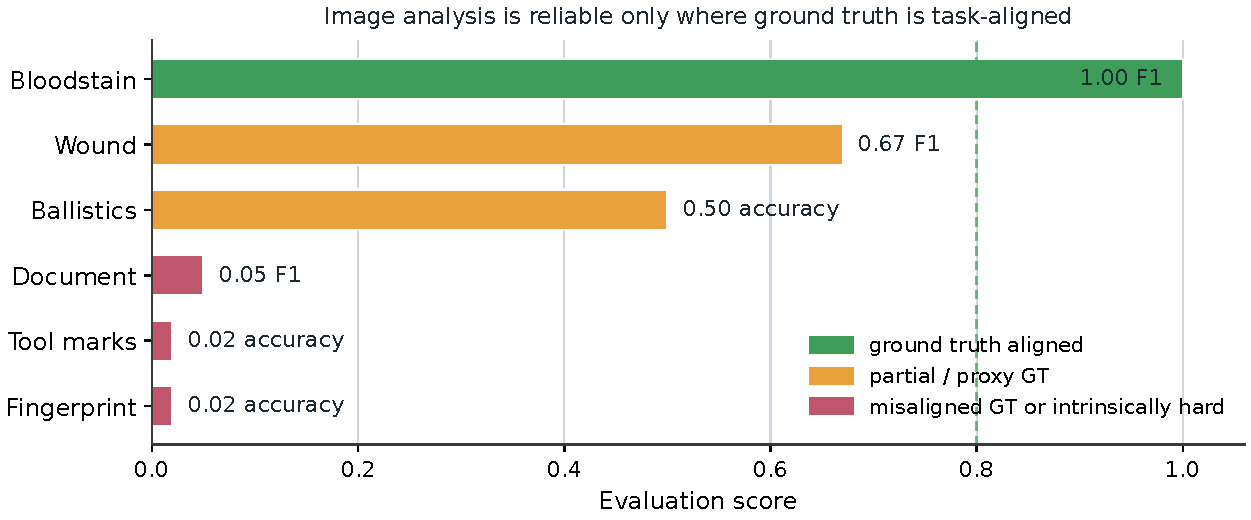
\includegraphics[width=\columnwidth]{image_eval_summary.pdf}
  \caption{Image analysis is reliable only where ground truth is task-aligned.
  Bloodstain (physics-grounded) succeeds; tasks with misaligned or proxy ground
  truth, or that are intrinsically hard from a single image, do not.}
  \label{fig:imgeval}
\end{figure}

\paragraph*{Hybrid ablation} On the full impact-spatter set ($n{=}61$) we ablate the
image pipeline into CV-only, LLM-only, and the full CV$+$LLM hybrid
(\cref{tab:bloodstainabl}). Classical CV features \emph{alone} produce no pattern
label, so CV-only detection is $\mathrm{F1}=0$: the CV stage extracts stain
geometry, not a semantic class. The LLM vision step alone detects impact spatter
on all $61$ samples ($\mathrm{F1}=1.0$), and the full hybrid matches it ($1.0$).
The honest reading is that the \emph{LLM} drives the high-level classification and
the CV stage is necessary only for the quantitative per-stain features it adds to
the graph; on this coarse binary metric the hybrid gains no accuracy over
LLM-only. This tempers, rather than supports, a strong hybrid claim on this task.

\begin{table}[t]
  \centering
  \caption{Bloodstain image ablation (impact-spatter detection, full set $n{=}61$).
  CV alone yields no semantic label; the LLM drives detection; the hybrid adds no
  accuracy over LLM-only on this coarse metric.}
  \label{tab:bloodstainabl}
  \footnotesize
  \begin{tabular}{@{}lc@{}}
    \toprule
    \textbf{Configuration} & \textbf{F1} \\
    \midrule
    CV-only (no LLM)        & 0.00 \\
    LLM-only (no CV)        & 1.00 \\
    CV\,$+$\,LLM (hybrid)   & 1.00 \\
    \bottomrule
  \end{tabular}
\end{table}

\subsection{Cross-case resolution (RQ4)}
\label{sec:res_eval}
We evaluate resolution over all $28$ cases and, to expose recall, label
\emph{every} candidate pair, not only the accepted ones (\cref{tab:resolution}).
In a single run, the $239$ resolvable entities admit $9973$ cross-case pairs;
embedding blocking keeps $243$; the conservative decision (\cref{eq:accept})
accepts $28$. \textbf{Precision is $27/28=0.96$}: the accepts comprise $16$
crime-type category links, $7$ recurring person/organisation identities, $3$
generic weapon-type links, and $1$ location. Crucially, the resolver recovers the
three \emph{genuine} shared-suspect links the dataset contains by
construction: the gang members \emph{Ravi Kapoor}, \emph{Amit Shukla}, and
\emph{Baljeet Malik}, shared by the Jigisha Ghosh and Soumya Vishwanathan murders
(confidence $0.80$, name-plus-context), plus the recurring Central Bureau of
Investigation (three cases) and Delhi Police. The \textbf{single false merge} is
instructive: a \emph{witness} ``Ajay Kumar'' in the Nitish Katara case is linked to
an \emph{accused} of the same common name in Soumya Vishwanathan, accepted on the
identical name alone (confidence $0.60$, the lowest of any accept) despite the role
disagreement, the bare-common-name collision the design tries to suppress. \textbf{Candidate-set recall is $0.15$} ($27$ of $178$ pool identities):
the $151$ misses are overwhelmingly identical crime types ($146$,
\emph{Murder}\,$=$\,\emph{Murder} across cases) the decision rejects for lacking
corroborating context, a deliberate choice not to link on a bare common word.
Candidate-set $\mathrm{F1}$ is thus $0.26$. This blended figure, however, mixes two
distinct tasks; separated, the forensically-relevant instance-identity recall is
$0.79$ at precision $0.92$ (\cref{tab:frontier}, discussed next), and the low
blended recall is an artefact of category normalization. This is a candidate-set,
not a global, benchmark (should-link labels follow the objective rule of
\cref{tab:resolution}; absolute recall is bounded by blocking). Links are
non-destructive, so a cross-case query traverses \rel{same\_as} edges without
collapsing provenance.

\begin{table}[t]
  \centering
  \caption{Cross-case \rel{same\_as} resolution over all $28$ cases (one
  extraction run). Every candidate pair was labelled by an objective cross-case
  identity rule.}
  \label{tab:resolution}
  \footnotesize
  \setlength{\tabcolsep}{4pt}
  \begin{tabular}{@{}P{5.4cm}r@{}}
    \toprule
    \textbf{Stage} & \textbf{Pairs} \\
    \midrule
    All cross-case pairs (same type)         & 9973 \\
    After embedding blocking (candidate pool) & 243 \\
    Accepted \rel{same\_as} links             & 28 \\
    \quad true accepts (TP)                   & 27 \\
    \quad false accepts / merges (FP)         & 1 \\
    True identities missed in pool (FN)       & 151 \\
    \midrule
    \multicolumn{2}{@{}l}{Candidate-set precision $0.96$, recall $0.15$, F1 $0.26$} \\
    \bottomrule
  \end{tabular}
\end{table}

\paragraph*{Instance identity vs.\ category normalization}
Cross-case \rel{same\_as} spans two tasks that should not share one recall number:
\emph{instance identity} (is \emph{Ravi Kapoor} in two cases the same person; is
this the recurring CBI?) and \emph{category normalization}, where every
\node{Murder} denotes the same crime \emph{class}. The blended candidate-set recall
of $0.15$ (\cref{tab:resolution}) conflates them, and is dominated by the $162$
category identities in the pool versus only $14$ instance identities. Separating
them (\cref{tab:frontier}) is far more informative. On the forensically-relevant
\textbf{instance-identity} task the deployed conservative resolver already attains
precision $0.92$ at candidate-set recall $0.79$ ($11/14$): it recovers the three
shared suspects (Ravi Kapoor, Amit Shukla, Baljeet Malik across the Jigisha Ghosh
and Soumya Vishwanathan cases), the recurring Central Bureau of Investigation and
Delhi Police, and the overlapping Vasant Kunj location, with a single common-name
false merge (``Ajay Kumar''). \textbf{Category normalization} is a separate, easier
task with no collision risk; the conservative rule's $0.10$ recall there is
over-cautious and is what depresses the blended figure. A \emph{type-aware tiered}
policy, which we propose rather than deploy, would auto-merge identical category
nodes (trivially reaching recall $1.0$ at precision $1.0$) and route identical
\emph{instance} names lacking corroboration to a human-review queue
($\approx\!0.1$ pairs/case), which \emph{would} recover the remaining instance
identities; the queue is a proposed operating mode, not an adjudicated automatic
result. We therefore report the conservative resolver as the deployed forensic
setting and the tier as a normalization/review variant. All recall here is
candidate-set (absolute recall remains bounded by the embedding-blocking floor).

\begin{table}[t]
  \centering
  \caption{Cross-case \rel{same\_as} \emph{by task type}: instance identity (the
  forensic task) reported separately from category normalization. Recall is
  candidate-set (bounded by blocking). \emph{Conservative} is the deployed
  resolver; \emph{tiered} is a proposed normalization\,$+$\,review variant
  (instance recall via a $\approx\!0.1$ pairs/case review queue).}
  \label{tab:frontier}
  \footnotesize
  \setlength{\tabcolsep}{5pt}
  \begin{tabular}{@{}P{3.9cm}cccc@{}}
    \toprule
     & \multicolumn{2}{c}{\textbf{Conservative}} & \multicolumn{2}{c}{\textbf{Tiered}} \\
    \cmidrule(lr){2-3}\cmidrule(lr){4-5}
    \textbf{Task} & \textbf{P} & \textbf{R} & \textbf{P} & \textbf{R} \\
    \midrule
    Instance identity (Person/Loc/Weapon) & 0.92 & 0.79 & 0.93 & 1.00 \\
    Category normalization (CrimeType)     & 1.00 & 0.10 & 1.00 & 1.00 \\
    \bottomrule
  \end{tabular}
\end{table}

\subsection{Error analysis}
\label{sec:erroranalysis}
\Cref{tab:errors} summarises the dominant, recurring error patterns; we report
patterns rather than cherry-picked instances. The dominant remaining error is a
single \emph{representation/matching} mismatch rather than a perception failure:
\node{Location} over-listing. The gold lists one principal location per case while
the extractor faithfully returns every place mentioned, so precision is $0.19$
though the principal location is recovered in $11/28$ cases. It is fixable by
binding the case to its principal event/location (via
\rel{happened\_on}/\rel{occurred\_at}) and scoring against that. Concretely, the
\node{Location} ``false positives'' are real, relevant places that are often
\emph{more specific} than the gold: for Abhaya the system extracts
\emph{``St Pius X Convent''} (the actual scene) against the gold's
\emph{``Kottayam''}; for Dabholkar, \emph{``Omkareshwar bridge''} against
\emph{``Pune''}; and for Gauri Lankesh, \emph{``the driveway of her home''}
against \emph{``Rajarajeshwari Nagar''}. These are not wrong, underscoring that
for \node{Location} the metric, not the extraction, is the limiting factor.

\node{TimeEvent} illustrates the same principle at the level of \emph{where} a
value is stored. The two-stage extractor records each event's calendar date in a
structured \texttt{date} field (e.g.\ \texttt{2017-09-05} for Gauri Lankesh) and
gives the node a descriptive name (\emph{``Murder of Gauri Lankesh''}); an
evaluation that read only the name scored \node{TimeEvent} at $\mathrm{F1}=0.09$
and date coverage at $0.10$, suggesting a recovery gap. Reading the field the
schema designates for dates, as the system itself does when querying, raises
\node{TimeEvent} to $0.88$ and date coverage to $0.95$. The dates were always
extracted; the earlier metric conflated schema \emph{location} with
non-recovery, precisely the validity confusion this paper warns against. (The
naive baseline, instructed to embed the date in the event name, scores $0.91$
either way.)

\begin{table}[t]
  \centering
  \caption{Representative error patterns by entity type (real-case set).}
  \label{tab:errors}
  \footnotesize
  \setlength{\tabcolsep}{3.5pt}
  \begin{tabular}{@{}P{1.5cm}P{2.6cm}P{3.0cm}@{}}
    \toprule
    \textbf{Type} & \textbf{Dominant error} & \textbf{Likely cause} \\
    \midrule
    Location  & over-listing; low precision & gold has 1 principal place; model lists all mentions \\
    TimeEvent & apparent low precision (metric only; resolved) & date stored in structured \texttt{date} field; name-only scoring under-counted \\
    Person    & occasional FN on minor actors & person named once in passing \\
    Weapon / method & rare FN & method stated narratively, not as a noun \\
    \bottomrule
  \end{tabular}
\end{table}

\subsection{Ablation: the value of ontology guidance}
\label{sec:ablation}
To isolate the contribution of ontology-guided extraction we compare the full
system against a baseline that uses the \emph{same} LLM and JSON output but a
single generic entity-extraction prompt (no forensic ontology type descriptions,
no per-type rules, and no two-stage relation grounding) scored by the
\emph{identical} matcher over the same 28 cases, three runs each
(\cref{fig:ablation}). The result is decisive. Ontology guidance is
what makes the \emph{structured forensic types} recoverable at all: it lifts
\node{Weapon}/method from $\mathrm{F1}=0.00$ to $0.72$ (the baseline records no
usable weapon across any case, never tagging, e.g., \emph{cyanide}, the Koodathayi
murder agent, as a \node{Weapon}/method, whereas the ontology-guided extractor
recovers weapons at recall $0.66$); it lifts \node{CrimeType} from $0.75$ to $0.91$
and \node{Location} from $0.13$ to $0.27$, and matches the baseline on
\node{Person} ($0.88$) and \node{TimeEvent} ($0.88$ vs.\ $0.91$). The full system
therefore wins on \emph{both} aggregate measures: macro-$\mathrm{F1}$
$0.73$ vs.\ $0.53$ and micro-$\mathrm{F1}$ $0.78$ vs.\ $0.68$. (An earlier
evaluation that scored \node{TimeEvent} from the event name alone
(\cref{sec:erroranalysis}) made the baseline appear to win micro-$\mathrm{F1}$;
reading the structured \texttt{date} field removes that artefact.) The honest
reading is that ontology guidance helps wherever forensic typing matters and costs
nothing on the types both systems already handle. A further
design choice with a \emph{measured} effect reported above is the label-free
evaluation fix that corrected a false fingerprint score from $100\%$ to
$\approx0\%$ (\cref{sec:setup}). A second ablation isolates the bloodstain image
pipeline (CV-only vs.\ LLM-only vs.\ CV$+$LLM), reported in \cref{sec:results}.
A \emph{third} ablation evaluates the NL-to-Cypher reasoning layer, the component
previously described but not measured, over $24$ factual questions on the populated
graph (\cref{tab:queryabl}). It compares the deployed \emph{grounded} generator
(the ontology schema in the prompt, over a graph normalised so every entity is
anchored to its case via the ontology-defined relationship, plus a Cypher
self-correction loop) against a \emph{naive} ungrounded LLM-to-Cypher baseline.
Grounding is decisive: answer correctness rises from $0.04$ to $\mathbf{0.67}$ and
schema hallucination, queries naming a node label or relationship type absent from
the graph, falls from $0.96$ to $\mathbf{0.04}$, while both produce executable
Cypher. The residual errors are concentrated in weapon questions, for which the
ontology defines no direct Case--Weapon edge (weapons attach via \rel{used\_weapon}
from a person/event); victim, accused, crime-type, location, and aggregate
questions are answered reliably. This fills the reasoning-layer evaluation gap and
quantifies why schema grounding and a case-anchored graph matter. The remaining
comparisons, removing the graph entirely and disabling resolution, are left to
future work (\cref{sec:future}).

\begin{table}[t]
  \centering
  \caption{Reasoning-layer ablation: graph-grounded vs.\ naive NL-to-Cypher over
  $24$ factual questions on the populated 28-case graph. Grounding (ontology schema
  $+$ case-anchored graph $+$ self-correction) nearly eliminates schema
  hallucination and lifts answer correctness $17\times$.}
  \label{tab:queryabl}
  \footnotesize
  \setlength{\tabcolsep}{5pt}
  \begin{tabular}{@{}P{4.6cm}ccc@{}}
    \toprule
    \textbf{NL\,$\to$\,Cypher method} & \textbf{Exec.} & \textbf{Correct} & \textbf{Halluc.} \\
    \midrule
    Naive (ungrounded, no schema)        & 1.00 & 0.04 & 0.96 \\
    Grounded (schema $+$ self-correction) & 1.00 & \textbf{0.67} & \textbf{0.04} \\
    \bottomrule
  \end{tabular}
\end{table}

\begin{figure}[t]
  \centering
  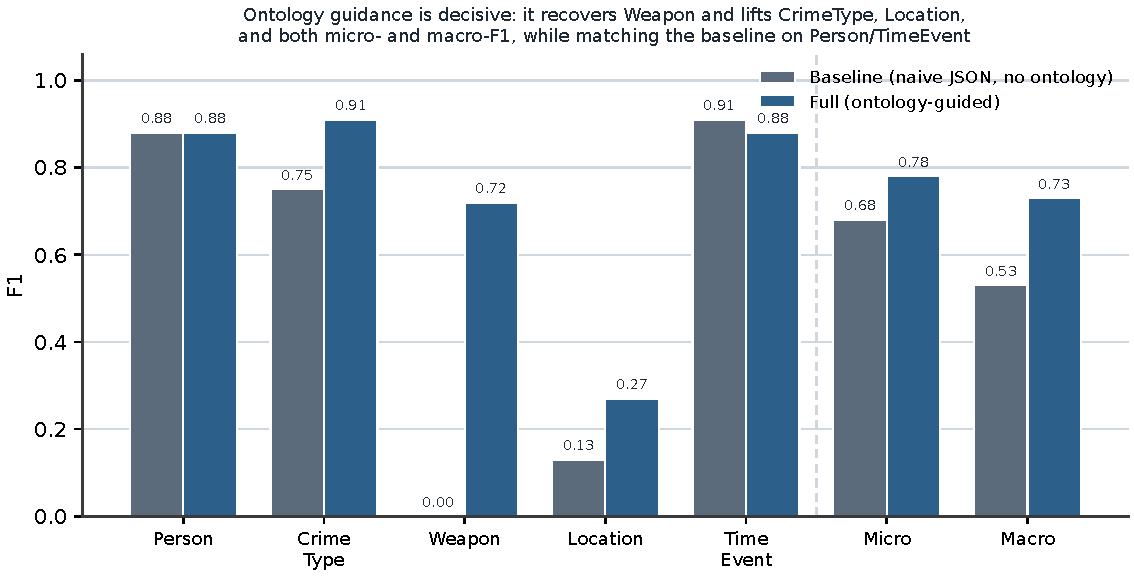
\includegraphics[width=\columnwidth]{ablation.pdf}
  \caption{Ablation: ontology-guided full system vs.\ a naive JSON baseline
  (same LLM, no ontology), F1 by type and overall, mean over three runs. Ontology
  guidance is decisive for \node{Weapon}, \node{CrimeType}, and \node{Location} and
  wins on both micro- and macro-F1, while matching the baseline on \node{Person}
  and \node{TimeEvent}.}
  \label{fig:ablation}
\end{figure}

% =====================================================================
\section{Discussion}
\label{sec:discussion}

\paragraph*{Why graph structure helps} Representing a case as a typed graph makes
the relationships that matter to investigation (who was involved, what caused
death, what preceded what, which evidence supports which hypothesis) explicit and
traversable. Multi-hop and cross-case questions become graph patterns rather than
brittle joins, and evidence chains become first-class objects that a human can
audit.

\paragraph*{Why real-case validation matters} Validating against documented facts
of real cases is the difference between measuring self-consistency and measuring
correctness. Our most defensible findings: stable recovery of persons, weapons,
and crime types ($\mathrm{F1}\approx0.86$--$0.88$, sd\,$\le0.03$) and the measured
ablation gain from ontology guidance, come from this protocol precisely because
the gold was not produced by an LLM.

\paragraph*{Why the location score is low} \node{Location} extraction remains
limited: the system reliably recovers valid \emph{mentioned} places but does not
reliably \emph{select} the single principal event location, so the gold's principal
location is diluted by genuinely-relevant secondary places counted as false
positives. This is \emph{both} an evaluation-granularity issue \emph{and} a real
modelling problem requiring explicit principal-location classification, not merely
a metric artefact. We take a first step (a gold-free first-mention selector recovers
the principal scene in $21/28$ cases, \cref{tab:locmetrics}), and binding the case
to its principal location via \rel{occurred\_at} and scoring against that is the
natural next step; but reliable principal-location selection is a genuine remaining
problem.

\paragraph*{Why image results contain negatives} The image negatives are
informative. They separate genuine model limitations (single-image forgery
detection is hard without an exemplar) from evaluation artefacts (fingerprint
``failure'' is really a ground-truth mismatch). Reporting both, instead of
selecting the one task that works, is what makes the bloodstain success
credible.

\paragraph*{Why non-destructive resolution is safer} In forensics a fabricated
connection can mislead an investigation. Linking rather than merging means the
system can surface a possible cross-case connection while preserving the ability
to reject it, and it never destroys the source provenance that an analyst needs
to evaluate the link.

\paragraph*{LLM hallucination and its mitigation} The framework mitigates
hallucination through four reinforcing mechanisms: ontology validation (typed
filtering of outputs), strict structured output (schema-constrained generation),
retrieval grounding (querying anchored in real labels and paths), and
evidence-chain reporting (every hypothesis cites its supporting nodes). None
eliminates hallucination, but together they bound it and make residual errors
visible and auditable.

% =====================================================================
\section{Threats to Validity}
\label{sec:threats}

\paragraph*{Internal validity} Extraction and scoring share fuzzy-matching
heuristics, so a lenient matcher could over-credit extraction. We mitigate this
with exact documented-fact gold, conservative matchers, and per-type reporting
that would expose leniency: location precision is reported low ($0.19$), not
masked. LLM stochasticity is a second internal threat: schema constraints bound,
but do not remove, run-to-run variance; we report mean\,$\pm$\,standard deviation
over three runs and a case-level bootstrap $95\%$ CI ($[0.74,0.82]$ for overall
micro-F1). The remaining gaps are listed as
future work: the full baseline matrix beyond the ontology ablation
(\cref{sec:ablation}) and a still larger, more routine case set. With $28$ cases
a formal significance claim would still be premature, so we present the numbers as
indicative.

\paragraph*{External validity} The $28$ real cases (and small per-modality image
samples) skew toward high-profile Indian cases; the results may not transfer to
routine casework, other jurisdictions, or other languages. Synthetic text is
deliberately excluded from our headline claims for exactly this reason
(\cref{sec:tracks}).

\paragraph*{Construct validity} Our metrics measure recovery of entities and
relations against documented facts: a proxy for, not a guarantee of, investigative
usefulness. The image negatives are partly a construct problem: a dataset label
(finger position) can fail to operationalise the intended construct (pattern
class), so a low score reflects measurement mismatch rather than model
incapability. Where the construct is well operationalised (bloodstain mechanism),
the same pipeline scores at ceiling.

\paragraph*{Ethical and legal validity} The framework produces hypothesis support,
not determinations. Any deployment raises privacy, bias, security, and
chain-of-custody concerns and would require expert oversight and governance. We
make no claim of forensic validity or legal admissibility, and no output should
serve as the sole basis for any investigative or legal decision.

% =====================================================================
\section{Limitations}
\label{sec:limitations}

We state limitations explicitly. The system should be treated as an exploratory
research prototype: no claim is made that extracted graph facts, \rel{same\_as}
links, or generated hypotheses meet forensic admissibility standards.
\textbf{(1)} The system is decision and hypothesis support, \emph{not} a
replacement for forensic experts, and we make no claim of forensic correctness
beyond the measured evidence, nor any claim of legal admissibility. \textbf{(2)} Extraction and reasoning depend on hosted LLMs,
which raises reproducibility concerns: outputs can vary across model versions and
sampling. \textbf{(3)} Access to real forensic data is limited; much of our
text data is synthetic and therefore weak for external validity, which is why we
foreground the real-case protocol. \textbf{(4)} Image tasks require
domain-aligned ground truth; several public datasets do not encode the attribute
the forensic task needs. \textbf{(5)} Single-image forensic interpretation is
intrinsically limited for comparison tasks (forgery, tool-mark, ballistic
matching) that need reference exemplars or multi-view evidence. \textbf{(6)}
Real-world deployment would require audit logging, security, privacy protection,
and expert review that are out of scope here. \textbf{(7)} Evaluation sample
sizes, 28 real cases and small per-modality image samples, remain limited, so
the reported numbers should be read as indicative rather than definitive.

% =====================================================================
\section{Future Work}
\label{sec:future}

Several directions follow directly. \emph{Powered, baselined evaluation} is the
immediate priority: completing the controlled component matrix beyond the three
ablations reported here (removing the graph entirely and
disabling resolution); and expanding real-case validation beyond 28 cases with
formal significance testing. \emph{Expert
annotation}: building on the faculty domain-plausibility review
(\cref{sec:facultyreview}), extend the two-annotator gold (\cref{sec:iaa}) with
forensic/legal \emph{practitioner} validation for rigorous, attribute-level review,
and add an explicit mapping between Indian legal categories (IPC/CrPC sections),
forensic-medical categories, and the graph node/relationship types. \emph{More real data}: incorporate larger
corpora of real FIR, police, and laboratory documents, and \emph{multilingual}
Indian legal and forensic text. \emph{Multi-view image evidence}: support
exemplar-based and multi-view comparison for forgery, tool-mark, and ballistic
tasks that single images cannot resolve. \emph{Domain-specific models}: distil
smaller, cheaper extraction models specialised to forensic schemas to improve
reproducibility and cost. \emph{Human-in-the-loop}: add annotation and active
learning so analyst corrections improve extraction over time. \emph{Uncertainty
calibration}: attach calibrated confidence to extracted facts and hypotheses.
\emph{Provenance and integrity}: add chain-of-custody-aware, versioned graph
provenance so that every node and edge carries an immutable, auditable history.

% =====================================================================
\section{Conclusion}
\label{sec:conclusion}

We presented an ontology-guided, multimodal forensic knowledge graph framework
that unifies heterogeneous legal, textual, and visual evidence into one
type-validated, embedded, queryable graph, with a reasoning layer for semantic
retrieval, grounded querying, temporal reconstruction, conservative
cross-case entity resolution, and auditable hypothesis support. On the documented
facts of 28 real Indian criminal cases (two-annotator gold, three runs each) the
framework recovers persons, crime types, weapons, and dated events strongly and
stably ($\mathrm{F1}=0.88$, $0.91$, $0.72$, $0.88$; sd\,$\le0.01$), with overall
micro-/macro-$\mathrm{F1}=0.78/0.73$ (bootstrap CI $[0.74,0.82]$); an ablation shows
ontology guidance is what makes the structured forensic types recoverable and lets
the full system lead on both micro- and macro-F1, with \node{Location} the one
remaining weak type. Image
analysis is reliable only where ground truth is task-aligned; we report the
remaining near-zero scores as evidence of evaluation honesty. We do not claim to
automate forensic judgement: the framework structures evidence and supports
hypotheses for a human expert, and establishing forensic validity would require
expert-annotated data and prospective study, which we leave to future work. Within
those bounds, the contribution is a reproducible framework and an evaluation
methodology, in particular a documented-fact protocol, that can help discourage
circular benchmarking in forensic AI.

% =====================================================================
\bibliographystyle{IEEEtran}
\bibliography{references}

% =====================================================================
% Appendix is placed after the bibliography so its wide \texttt{table*}
% (\cref{tab:cases}) can never float into and interrupt the reference list.
\appendix
\label{sec:appendix}

\subsection{Real-case list and gold-curation protocol}
\label{app:cases}
\Cref{tab:cases} lists the 28 documented cases and the composition of their gold
(counts of gold Person/Location/Weapon/TimeEvent entries). Gold annotations were
curated from authoritative public records, the English-language encyclopedic
summary of each case and contemporaneous court reporting, by a first annotator,
who dropped two unnatural-death cases (the Burari deaths and the Sunanda Pushkar
death) whose ``crime type'' does not map to a canonical category and normalised
entries (name spellings, the choice of principal location, weapon/method). A
second annotator then independently re-annotated all 28 cases from the narratives,
blind to the first annotator's labels; the two annotations agree at Cohen's
$\kappa=0.95$ on roles and $1.0$ on crime type (\cref{sec:iaa}, \cref{tab:iaa}),
validating the first annotator's curation as the gold used here (the full
disagreement list is released).
For each case we recorded the named persons and their roles, the single principal
location, the weapon or method, the crime type(s), and the documented
dates/time-events, recording only facts asserted by the sources and not
inferences. The pipeline is run on a short factual narrative of each case
(distinct from the gold) and scored against these facts. The bias toward
high-profile, well-documented cases remains a limitation (\cref{sec:threats}); a
still broader, less self-selected case set would further strengthen external
validity.

\begin{table*}[t]
  \centering
  \caption{The 28 documented real cases (two-annotator gold), gold composition
  (P/L/W/T = gold Person/Location/Weapon/TimeEvent counts), and per-case
  full-system F1 (mean over three runs), sorted by F1. Sources are the
  corresponding English Wikipedia articles and contemporaneous court reporting.}
  \label{tab:cases}
  \scriptsize
  \renewcommand{\arraystretch}{0.96}
  \setlength{\tabcolsep}{4pt}
  \begin{tabular}{@{}P{3.7cm}ccccc@{\hspace{1.2cm}}P{3.7cm}ccccc@{}}
    \toprule
    \textbf{Case} & \textbf{P} & \textbf{L} & \textbf{W} & \textbf{T} & \textbf{F1} &
    \textbf{Case} & \textbf{P} & \textbf{L} & \textbf{W} & \textbf{T} & \textbf{F1} \\
    \midrule
    Murder of Narendra Dabholkar   & 3 & 1 & 1 & 2 & 0.94 & Murder of Soumya Vishwanathan   & 6 & 1 & 1 & 2 & 0.78 \\
    Murder of Gauri Lankesh        & 3 & 1 & 1 & 1 & 0.88 & Swathi murder case              & 2 & 1 & 1 & 3 & 0.78 \\
    Koodathayi cyanide killings    & 10 & 1 & 1 & 6 & 0.88 & 2008 Aarushi--Hemraj murder     & 4 & 1 & 2 & 4 & 0.77 \\
    Assassination of Phoolan Devi  & 2 & 1 & 1 & 2 & 0.88 & Kathua rape \& murder           & 4 & 1 & 2 & 3 & 0.77 \\
    Murder of Jigisha Ghosh        & 4 & 1 & 0 & 3 & 0.87 & Murder of Pradyuman Thakur      & 2 & 1 & 1 & 1 & 0.75 \\
    Murder of Priyadarshini Mattoo & 2 & 1 & 2 & 3 & 0.87 & Nithari serial murders          & 3 & 1 & 1 & 4 & 0.73 \\
    2012 Delhi gang rape \& murder & 8 & 1 & 1 & 3 & 0.87 & Saravana Bhavan (Santhakumar)   & 3 & 1 & 0 & 3 & 0.73 \\
    Tandoor murder (Naina Sahni)   & 4 & 1 & 1 & 4 & 0.83 & 2020 Hathras gang rape \& murder & 4 & 1 & 0 & 3 & 0.72 \\
    Murder of Jessica Lal          & 4 & 1 & 1 & 3 & 0.82 & Murder of Graham Staines        & 5 & 1 & 1 & 2 & 0.70 \\
    Murder of Neeraj Grover        & 3 & 1 & 1 & 2 & 0.82 & Bilkis Bano case                & 2 & 1 & 3 & 3 & 0.67 \\
    Murder of Pramod Mahajan       & 2 & 1 & 1 & 3 & 0.82 & 2024 R.\,G.\,Kar rape \& murder  & 2 & 1 & 1 & 3 & 0.67 \\
    Sister Abhaya murder           & 3 & 1 & 1 & 2 & 0.78 & Murder of Shraddha Walkar       & 2 & 1 & 1 & 2 & 0.67 \\
    1999 Delhi BMW hit-and-run     & 6 & 1 & 1 & 2 & 0.78 & Nitish Katara murder            & 8 & 1 & 1 & 3 & 0.61 \\
    Murder of Sheena Bora          & 5 & 1 & 1 & 2 & 0.78 & Soumya murder case (train)      & 2 & 1 & 0 & 2 & 0.60 \\
    \midrule
    \multicolumn{12}{@{}l}{\textbf{Totals:} 108 Person, 28 Location, 29 Weapon, 76 TimeEvent gold entries across 28 cases; \textbf{mean per-case F1 $=0.78$} (range $0.60$--$0.94$).} \\
    \bottomrule
  \end{tabular}
\end{table*}

\subsection{Ontology and relationship summary}
\Cref{tab:ontology} lists node groups; the 48 relationship types fall into
involvement, spatial/temporal, causal/medical, evidential, image-derived, and
cross-case families. Controlled enumerations (e.g.\ \texttt{PatternType},
\texttt{InjuryType}, \texttt{FingerprintClass}, \texttt{ToolMarkType}) constrain
selected attributes at insertion.

\subsection{Baseline extractor (ablation)}
\label{app:baseline}
The naive baseline of \cref{sec:ablation} uses the same model and JSON output as
the full system but a single generic prompt with no ontology type descriptions,
no per-type rules, and no two-stage relation pass. It asks the model to extract
entities of type \node{Person}, \node{Location}, \node{Weapon}, \node{CrimeType},
\node{TimeEvent}, or \node{Case} from the factual narrative into JSON
(\texttt{\{entity\_type, properties\}}), with \node{Person} carrying name and role
and the others a name/type, and nothing about the forensic ontology,
relationships, or evidence spans. Both conditions are scored by the identical
matcher; the released experiment script contains the exact prompt.

\subsection{Structured extraction schema (illustrative)}
Entity extraction emits objects of the form
\texttt{\{entity\_type, entity\_id, properties\}} constrained to a per-document
JSON schema; relationship extraction emits
\texttt{\{source\_entity\_id, target\_entity\_id, relationship\_type,}
\texttt{confidence, evidence\_span\}}, where \texttt{evidence\_span} is the exact
supporting text. Identifiers are namespaced per document to prevent cross-document
collisions.

\subsection{Example Cypher query}
A grounded NL-to-Cypher generation for ``which cases share a cause of death linked
to the victim?'' yields a pattern such as:
\begin{quote}\footnotesize\ttfamily
MATCH (c:Case)<-[:INVOLVED\_IN]-(p:Person)\\
\hspace*{1em}<-[:CAUSE\_OF\_DEATH\_OF]-(cod:CauseOfDeath)\\
RETURN c.title, p.name, cod.primary\_cause LIMIT 50
\end{quote}

\subsection{Ethical considerations}
This framework is intended for research and as decision/hypothesis support under
expert oversight. It must not be used as a sole basis for any legal or
investigative determination. Deployment on real case data would require informed
governance, access control, privacy safeguards, bias assessment, and human expert
review. Reported metrics describe performance on the stated datasets only and do
not constitute a claim of forensic validity or legal admissibility.

% =====================================================================
\end{document}
